\documentclass[a4paper,12pt]{article}
\usepackage{latexsym}
\usepackage{array}
\usepackage{amsmath}
\usepackage{amsfonts}
\usepackage{amssymb}
\usepackage{mathrsfs}
\usepackage{graphicx}
\usepackage{bm}
\usepackage{braket}
\usepackage{subfigure}
\usepackage{color}
\usepackage{colortbl}
\usepackage{cite}
\usepackage{float}
\usepackage{eqparbox}
\usepackage{graphicx}
\usepackage{ulem}
\usepackage{booktabs}
\usepackage[Symbol]{upgreek}
\usepackage{subfigure}
\usepackage{stfloats}
\usepackage{algorithmicx,algorithm}
\usepackage[noend]{algpseudocode}
\usepackage{threeparttable}
\usepackage{theorem}
\usepackage{times}
\usepackage{dcolumn}
\usepackage{bbm}
\usepackage{multirow}
%\usepackage[boxed]{algorithm2e}
\usepackage{framed}
\usepackage{xcolor}
\usepackage{lipsum}
\usepackage{soul}
\usepackage{mdframed}

\renewcommand{\algorithmiccomment}[1]{\hfill\eqparbox{COMMENT}{\%~#1}}

\newtheorem{theorem}{\bf Theorem}
\newtheorem{proposition}{\bf Proposition}
\newtheorem{lemma}{\bf Lemma}
\newtheorem{definition}{Definition}
\newtheorem{remark}{\bf Remark}


\setlength{\textheight}{245mm}
\setlength{\textwidth}{170mm}
\setlength{\topmargin}{-15mm}
\setlength{\oddsidemargin}{-5mm}
\setlength{\evensidemargin}{-5mm}
\flushbottom
\setlength{\parindent}{0pt}
\setlength{\baselineskip}{17pt}
\setlength{\parskip}{3mm}
\setlength{\columnsep}{8mm}
\renewcommand{\baselinestretch}{1.3}
\hyphenation{op-tical net-works semi-conduc-tor IEEEtran}
\DeclareGraphicsRule{.png}{eps}{.bb}{}
\allowdisplaybreaks[4]

\newcommand{\PreserveBackslash}[1]{\let\temp=\\#1\let\\=\temp}
\newcommand{\red}[1]{{\color{red}{#1}}}
\newcommand{\blue}[1]{{\color{blue}{#1}}}
\newcommand{\Authors}[1]{{\blue{{\textbf{Authors: }}{#1}}}}

\newenvironment{cframed}[1][blue]
  {\def\FrameCommand{\fboxsep=\FrameSep\fcolorbox{#1}{white}}%
    \MakeFramed {\advance\hsize-\width \FrameRestore}}
  {\endMakeFramed}

\newenvironment{IEEEproof}{{\it Proof. }}{}
\newcolumntype{C}[1]{>{\PreserveBackslash\centering}p{#1}}
\newcolumntype{R}[1]{>{\PreserveBackslash\raggedleft}p{#1}}
\newcolumntype{L}[1]{>{\PreserveBackslash\raggedright}p{#1}}

\def \T {^{\mathsf{T}}}
\def \H {^{\mathsf{H}}}
\def \ri {{\rm i}}
\def \d {{\rm d}}

\def\onecol{}

\begin{document}

\begin{center}
 {\Large\bf A General DoF and Pattern Analyzing Scheme for Electromagnetic Information Theory}
\end{center}
\begin{center}
 {\Large\bf (Original paper ID: IT-25-0327)}
\end{center}
\begin{center}
 {\Large\bf Response Letter}
\end{center}
\begin{center}
Zhongzhichao Wan, {\it Student Member,~IEEE}, Jieao Zhu, {\it Student Member,~IEEE}, \\Yongli~Yan, {\it Member,~IEEE}, and Linglong Dai, {\it Fellow,~IEEE}

\end{center}
\vspace*{+2mm}
\begin{center}
 {\Large\bf Response to Editor's Comments}
\end{center}


\textbf{Editor}: Manuscript ID IT-25-0327 titled "A General DoF and Pattern Analyzing Scheme for Electromagnetic Information Theory" which you submitted to the IEEE Transactions on Information Theory, has been reviewed.  The comments of the reviewer(s) are included at the bottom of this letter. There may be additional comments as separate files available through your Author Center on the ScholarOne Manuscripts web site, so please check there also to make sure you have received all reviewer comments.

\quad Based on my own detailed reading of the paper and the reviewers’ comments, I recommend that you revise and resubmit your manuscript. Specifically, in your revision, the following points must be addressed:

\quad The reviewers appreciate the generalization of the Slepian concentration theory to 3D and 4D domains. However, based on the reviews and my own reading, there seems to be some disconnection or potentially contradictions in the nature of the work that needs to be clarified or resolved. One of the main claims is the non-asymptotic analysis and as one reviewer has mentioned, to obtain the results, asymptotic analysis is needed. In that case, the justification for DoF analysis when capacity is understood is unclear. There are additional valuable comments from the reviewers.


\blue{
    {\bf Authors:}
    We would like to commence by thanking the editor and three professional reviewers for their valuable time in evaluating our submission. Your constructive comments and expert knowledge of the field have helped us to strengthen the manuscript significantly. We endeavored to address all the suggestions and comments, and our reflections are provided below in a point-to-point manner. We also indicate how our manuscript has been revised accordingly, and all the revisions have been highlighted in \red{red} color in the revised paper. Here, we would like to make a brief summary of the major revisions in the revised paper as below:
    \begin{enumerate}
    	\item a
%        \item To answer the relationship of our work with respect to existing works and show the novelty of our work, we have reorganized the contribution part in the Introduction section. 
%        \item To make the model more solid and persuasive, we have added explanations about the assumptions and simplifications used in the modeling part. We also show that some simplifications have already been adopted in existing papers.
%        \item To show the fitness of the model to practical scenarios, we have generated a channel based on Hong Kong streets using ray tracing, and then show the fitness of our model to it. 
%        \item We have also modified or rewritten several parts and added explanations to improve the readability of our paper.
    \end{enumerate}
}


{\bf Editor:} My own comments:

\quad As always the submission of the revised manuscript should be accompanied by a detailed response to the reviewers’ and to my comments.  In preparing this response, please pay particular attention to the points mentioned above.

\quad Once the revised manuscript is prepared, you can upload it and submit it through your Author Center.


\blue{
    {\bf Authors}:
    Many thanks again for Editor's and all the Reviewer's valuable time and efforts to review this paper. Based on your constructive comments, we have already made a careful major revision of this paper, which is attached to the end of this letter. 
    \\
    \\
    Sincerely, 

    {\it The Authors}
}

\clearpage


\begin{center}
    {\Large\bf Response to Reviewer 1's Comments}
\end{center}

{\textbf{Reviewer 1:}}
This paper provides a general scheme, where tools from Slepian concentration problem are used and extended to 3-dim space domain and 4-dim space-time domain, to analyze the (functional and channel) DoF of electromagnetic fields.

\quad I am not familiar with the subject of electromagnetic information theory, thus, I can only provide some minor comments.

{\color{blue}{\textbf{Authors: } 
We appreciate the reviewer's positive evaluations of our work. We have tried our best to revise the paper according to the reviewer's valuable comments, and our responses are provided in a point-to-point manner as below. 
}}

\textbf{Reviewer 1:}
1. In page 5, the last line above Eq. (3), the idea is perfectly fine but maybe it is a typo? From my limited understanding, for bandlimited functions, the $\lambda$ to be maximized should be
$\frac{\int_{-T}^T|g(t)|^2dt}{\int_{-\infty}^\infty|g(t)|^2dt}$?


{\color{blue}{\textbf{Authors: } 
Many thanks for the reviewer's valuable comment. $\{\lambda\}$ can be obtained both from time and frequency domain. The results will be the same. This phenomenon is ensured by Theorem 1 in the paper which comes from [26]. To be more straightforward, it shows some kind of "symmetry" on the two domains when finding the "most concentrated functions". In Eq. (3) we choose to have band-limitation in time domain (in another word we can say we observe the signal on a given time interval) and express $\lambda$ using frequency domain. The inverse procedure also exists and will lead to the same result. According to your comment, we have added more explanations in the paper. 

\quad Detailed revisions are shown in the following box:

}}
\begin{framed}
	{\bf Section II}

    
\end{framed}



\textbf{Reviewer 1:}
2. In page 9, the 4th line below Eq. (26), it should be “importance” instead of ”importance”.

{\color{blue}{\textbf{Authors: } 
Thanks for the reviewer for pointing out this problem. We have corrected this issue, the detailed revisions are shown in the following box.
}}

\begin{framed}
	{\bf Section III.A}

  

\end{framed}

\textbf{Reviewer 1:}
3. It is better to have some references for the last sentence of page 9. 

{\color{blue}{\textbf{Authors: } 
Thanks for the reviewer's valuable suggestions. We have added references that have restrictions on the wavenumber domain, which constraint the direction of the incident wave to the receiver. Such constraints affect the channel model and DoF analyzing results. Detailed revisions are shown in the following box.
}}

\begin{framed}
	{\bf Section IV.A}

    
\end{framed}

{\color{blue} \textbf{Authors}: Thank you for your valuable time and efforts to review this paper. Your comments and suggestions have helped us improve our work.
	\\
	\\
	Sincerely,
	
	{\it The Authors}
}


\clearpage

%%%%%%%%%%%%%%%%%%%%%%%%%%%%%%%%%%%%%%%%%%%%%%%%%%%%%%%%%%%%%%%%%%%%%%%%%%%%%%%%%%%%%
%%%%%%%%%%%%%%%%%%%%%%%%%%%%%%%%%%%%%%%%%%%%%%%%%%%%%%%%%%%%%%%%%%%%%%%%%%%%%%%%%%%%%
%%%%%%%%%%%%%%%%%%%%%%%%%%%%%%%%%%%%%%%%%%%%%%%%%%%%%%%%%%%%%%%%%%%%%%%%%%%%%%%%%%%%%
%%%%%%%%%%%%%%%%%%%%%%%%%%%%%%%%%%%%%%%%%%%%%%%%%%%%%%%%%%%%%%%%%%%%%%%%%%%%%%%%%%%%%

\begin{center}
    {\Large\bf Response to Reviewer 2's Comments}
\end{center}

\textbf{Reviewer 2:}
The paper focuses on the DoF for electromagnetic information theory under a non-asymptotic setting, i.e., finite spatial regions and finite frequency bandwidth. Building upon the Slepian concentration problem in one and two-dimensional domains, the asymptotic DoF in the three-dimensional space domain and the four-dimensional space-time domain under electromagnetic constraints is analyzed. Most importantly, it was proved that the channel DoF is upper bounded by the functional DoF of electromagnetic fields under a maximum error constraint. Numerical results show the impacts of the constraints on the space and wavenumber domains on the DoF. The reviewer appreciates the efforts that have been made to characterize the DoF of electromagnetic fields in a larger domain. However, the analysis is limited to the asymptotic case as it still requires the product of those domains to go to infinity to achieve the maximum DoF. In contrast, the non-asymptotic case is discussed in the numerical results only. In terms of the writing, the first half of the paper lacks a connection to information theory. The reviewer feels that the paper may be more suitable for journals like TCOM or TWC rather than T-IT. The detailed comments and suggestions are as follows.


{\color{blue}{\textbf{Authors: } 
We appreciate the reviewer's positive evaluations on our work. We have tried our best to revise the paper according to the reviewer's valuable comments, and our responses are provided in a point-to-point manner as below. 
}}


\textbf{Reviewer 2:}
1. As the authors pointed out, the capacity analysis of EIT has already been available in the literature. What is the motivation for studying the DoF? Isn’t the DoF a more restricted result compared to the capacity or mutual information analysis?

{\color{blue}{\textbf{Authors: } 
 Thanks to the reviewer's valuable comments. The motivation of studying the DoF can be presented from the following two perspectives: 1) The degrees of freedom (DoF) of an electromagnetic field characterize the dimension of the functional space it spans, i.e., the minimum number of orthogonal base functions required for its representation. Compared to mutual information or capacity analysis, the DoF analyzing framework offers a more fundamental and physically intuitive criterion for determining the number of antennas required in array design to approach optimal system performance. 2) While capacity and mutual information analysis in existing works rely on a specific channel model, in this paper the fDoF analysis is an upperbound covering all kinds of channel conditions, which only relies on the characteristics of the transceivers and is different from the results obtained from capacity or mutual information analysis. We have also discussed the relationship between fDoF and cDoF which relies on a specific channel. Therefore, our analysis about DoF has provided some new insights compared to existing capacity or mutual information analysis.  
 
 
  According to the reviewer's comments, we have added clarifications and explanations about the necessity of analyzing the DoF. The detailed revisions are shown in the following box:
}}

\begin{framed}
    {\bf Section II}

	\setcounter{equation}{0}

   
\end{framed}

\textbf{Reviewer 2:}
2. Upon reading half of the paper, it seems that the connection between the presented materials and information theory is lacking. The reviewer suggests reorganizing the paper and introducing relevant background on EIT or channel model, problem formulation, etc., in Section II first. For example, the authors could clarify the relation between the DoF and capacity in EIT.

{\color{blue}{\textbf{Authors: } 
Many thanks for the reviewer's valuable comment. Our equation here comes from the scalar wave equation as adopted by [20-24]. We agree with the reviewer that our derivation process in the paper is not clear and strict enough, where some items in the electromagnetic equations are ignored without discussion when using the scalar wave equation. We now begin from the vector wave equation form in [19], which includes the missing considerations when using scalar wave equation.

\quad Detailed revisions are shown in the following box:

}}
\begin{framed}
	{\bf Section II}

	\setcounter{equation}{0}

    \quad Maxwell's equations are the fundamental physical laws of the electromagnetic system. For the characteristics of the scattering system, we can consider the scatterers as spatial non-uniformity of the electromagnetic characteristics like permittivity $\epsilon$ and permeability $\mu$. {\color{red}We adopt the time-harmonic assumption which assumes that the electromagnetic waves oscillates on a single frequency point. Then we have ${\bf E}({\bf r},t) = {\bf E}({\bf r})e^{-{\rm j}\omega t}$, and the partial derivative $\partial/\partial t$ can be replaced by $-{\rm j}\omega$ [26].
Then from the Maxwell's equations we have}
\begin{subequations}
	\begin{align} 
		&\nabla \times {\bf E}({\bf r}) = {\rm j}\omega \mu({\bf r}) {\bf H}({\bf r}), \label{maxwell_1}\\
		& \nabla \times {\bf H}({\bf r}) = -{\rm j}\omega \epsilon({\bf r}) {\bf E}({\bf r})+{\bf J}({\bf r}),  \label{maxwell_2}\\
		& \nabla \cdot  (\epsilon({\bf r}) {\bf E}({\bf r})) = \rho({\bf r}),\\
		& \nabla \cdot (\mu({\bf r}) {\bf H}({\bf r})) = 0,
	\end{align}
\end{subequations}
where $\epsilon({\bf r})$, ${\mu}({\bf r})$ and $\rho({\bf r})$ represents the permittivity, permeability and charge density at the position ${\bf r}$. In homogeneous media, $\epsilon({\bf r})$ and ${\mu}({\bf r})$ will be constant, which is often used in light-of-sight channel modeling in the free space. Now we are considering inhomogeneous media, which can express the electromagnetic characteristics of scattering fields [19]. 

{\color{red}
	\quad By performing $\nabla\times$ on (1a), we have
	\begin{equation}
		\nabla \times \mu({\bf r})^{-1} \nabla \times {\bf E}({\bf r}) = \nabla \times ({\rm j}\omega{\bf H}({\bf r})),
	\end{equation}
	 which leads to the corresponding vector wave equation
	 \begin{equation}
	 	\nabla \times \mu({\bf r})^{-1} \nabla \times {\bf E}({\bf r}) - \omega^2 \epsilon({\bf r})  {\bf E}({\bf r}) = {\rm j}\omega {\bf J}({\bf r}),
	 \end{equation}
	 where $k({\bf r}) = \omega \sqrt{\mu({\bf r})\epsilon({\bf r})}$ represents the inhomogeneous media over a finite domain $V$ according to [19], and ${\rm j}\omega {\bf J}({\bf r})$ represents the source field. Outside the domain $V$, the wavenumber $k({\bf r})$ equals $k_0 = \omega\sqrt{\mu_0\epsilon_0}$.
	 By subtracting $\nabla \times \mu_0 \nabla  \times {\bf E}({\bf r})- \omega^2 \epsilon_0 {\bf E}({\bf r})$ from both sides and applying the Green's function, the received electric field can be expressed by
\begin{equation}
	\begin{aligned} 
		{\bf E}({\bf r}) &= {\rm j}\omega\int_{V_s} {\bf G}({\bf r},{\bf r}')\mu_0{\bf J}({\bf r}'){\rm d}{\bf r}' 
		+ \int_{V} {\bf G}({\bf r},{\bf r}')(k^2({\bf r}')-k_0^2) 
		{\bf E}({\bf r}'){\rm d}{\bf r}',
	\end{aligned}
	\label{equ_scattering_field}
\end{equation}
where $V_s$ is the source region which generates the signal, ${\bf E}({\bf r}')$ is the induced electric field in the inhomogeneous regions in the space, and the dyadic Green's function ${\bf G}$ is the solution of the equation
\begin{equation}
	\begin{aligned} 
		\nabla \times \mu_0^{-1} \nabla \times {\bf G}({\bf r},{\bf r}') - \omega^2 \epsilon_0  {\bf G}({\bf r},{\bf r}') = \mu_0^{-1} {\bf I} \delta({\bf r}-{\bf r}').
	\end{aligned}
\end{equation}
Then, we can obtain the Green's function as ${\bf G}({\bf r},{\bf r}') = \frac{1}{{4\pi }} \left( {{\bf{I}} + \frac{{{\nabla _{\bf{r}}}\nabla _{\bf{r}}^{\rm{H}}}}{{{\kappa_0 ^2}}}} \right) \frac{{{e^{{\rm{j}}\kappa_0 \left\| {{\bf{r}} - {\bf{r}'}} \right\|}}}}{{\left\| {{\bf{r}} - {\bf{r}'}} \right\|}} $, which can be further expressed by [27]:
\begin{equation}
	\begin{aligned}
		{\bf{G}}({\bf{r}},{\bf{r}'}) =& \frac{1}{{4\pi }}\frac{{{e^{{\rm{j}}\kappa_0 \left\| {{\bf{r}} - {\bf{r}'}} \right\|}}}}{{\left\| {{\bf{r}} - {\bf{r}'}} \right\|}}\Bigg[\left( {{\bf{I}} - {\bf{\hat p}}{{{\bf{\hat p}}}^{\rm{H}}}} \right) + \frac{{\rm j}}{2\pi \left\| {{\bf{r}} - {\bf{r}'}} \right\| /\lambda}\left( {\bf I}-3{\bf{\hat p}}{{{\bf{\hat p}}}^{\rm{H}}} \right) \\&-\frac{1}{(2\pi\left\| {{\bf{r}} - {\bf{r}'}} \right\|/\lambda )^2 }\left( {\bf I}-3{\bf{\hat p}}{{{\bf{\hat p}}}^{\rm{H}}}  \right) \Bigg] [{\rm m}^{-1}],
		\label{Green}
	\end{aligned}
\end{equation}
where ${\bf{\hat p}} = \frac{{\bf{r}} - {\bf{r}'}}{{\left\| {\bf{r}} - {\bf{r}'} \right\|}}$.
Here we assume that $\left\| {{\bf{r}} - {\bf{r}'}} \right\|/\lambda \gg 1$, which means that the receiver is in far-field of the scatterer's microstructure and holds true in general wireless communication scenarios [28]. Then, we can omit the items containing powers of $\frac{1}{\left\| {{\bf{r}} - {\bf{r}'}} \right\|/\lambda}$. Since ${\rm tr}({\bf I}-{\bf{\hat p}}{{{\bf{\hat p}}}^{\rm{H}}})({\bf I}-{\bf{\hat p}}{{{\bf{\hat p}}}^{\rm{H}}})^{\rm H} = 2$ is a constant, the average power of the electromagnetic field does not depend on the direction ${\bf{\hat p}}$ if the energy of the source current is equally distributed in all polarization directions. Then for simplicity in this paper we reduce the vector wave field to scalar wave field showing the power of electric field averaged on all polarization directions\footnote{\color{red}Physically if we consider the electromagnetic fields on a specific polarization direction $\hat{\bf a}$, an extra factor $\hat{\bf a}({\bf{I}} - {\bf{\hat p}}{{{\bf{\hat p}}}^{\rm{H}}})\hat{\bf a}^{\rm H}$ should be added.}. We have
\begin{equation}
	\begin{aligned} 
		E({\bf r}) =& {\rm j}\omega\mu_0\int_{V_s} g({\bf r},{\bf r}')J({\bf r}'){\rm d}{\bf r}' + \int_{V} g({\bf r},{\bf r}')(k^2({\bf r}')-k_0^2) 
		E({\bf r}'){\rm d}{\bf r}',
	\end{aligned}
	\label{equ_scattering_field_scalar}
\end{equation}		
where $g({\bf r},{\bf r}') = \frac{1}{2\pi}\frac{e^{{\rm j}k_0\| {\bf r}-{\bf r}' \|}}{\|{\bf r}-{\bf r}' \|}$.
}
The equation (\ref{equ_scattering_field_scalar}) is an extension from the 2-dimensional case in [29]. Here we can view the first item in (\ref{equ_scattering_field}) as the line-of-sight component of the field which is fixed and well-studied. Then we will focus on the second item in (\ref{equ_scattering_field}) which highly relies on the characteristics of the inhomogeneity of the space. The inhomogeneity of the space depends on the complicated factors such as surface structure and material properties of the medium which are hard to analytically model and may change over time. Therefore, a statistical model will be more suitable to depict the characteristics of the field than deterministic modeling scheme. 
\end{framed}

\textbf{Reviewer 2:}
The field inside the scattering integral is the 'internal' field generated by the field incident on the object. Estimation of the internal field is the hardest part of scattering problems. In Eq. 5, the authors suppose impulse spatial autocorrelations of the field induced in the scattering object. Using this approximation, all the scattering characteristics of the formula are lost, and the model becomes an electromagnetic 'source', and some mathematical approximations substitute the physics of the problem. This is fine, but in some way, all the discussion before is 'lost' when the authors arrive at Eq. 5.

{\color{blue}{\textbf{Authors: } 
Thanks for the reviewer's valuable comment. Choosing impulse spatial correlations is mainly for mathematical simplicity, and it has also been used in several existing papers, including [31-33]. According to the reviewer's suggestion, we list the different modeling schemes of the spatial correlation of the scattering field in the paper to better explain our modeling assumptions.

\quad Detailed revisions are shown in the following box:
}}

\begin{framed}
	{\bf Section III.A}

    To derive a closed-form expression of the channel model we need to have some assumptions on the scattering field to do simplifications on (8). {\color{red} Considering the uncertainty of the inhomogeneity of the space, simplified models need to be used for the field correlation on the scatter surfaces for ease of analysis. In the literature, some models have been already proposed. For example, delta function type of field spatial correlation is discussed in [31], [32] and [33], which implies an ideal but mathematically friendly assumption that the material properties are varying instantaneously in the spatial domain. A more complex model like exponential type of field spatial correlation is discussed in [34]. Angular delta function as the spectrum of the field is proposed in [35]. For simplicity, we adopt delta function as the spatial correlation of the fields on the scattering surface, leading to $\mathbb{E}\left[ E({\bf r}_1')E^{*}({\bf r}_2') \right] = \beta \delta({\bf r}_1'-{\bf r}_2')$.}

\end{framed}

\textbf{Reviewer 2:}
In Lemma 2 the distance d depends on $(r_s^2+r_m^2)$. The source and scattering objects represent two field sources whose global dimension is $(r_s+r_m)$. Consequently, one would expect d to depend on $(r_s+r_m)^2$. Please check the statement.

{\color{blue}{\textbf{Authors: } 
Thanks to the reviewer for pointing out this problem. We have checked the corresponding analysis. When we do simplification, some items are wrongly ignored. Then we revise the corresponding parts.
 Detailed revisions are shown as in the following box: 
}}
\begin{framed}
    {\bf Section IV. C}

    {\bf Lemma 2}(Extension of Rayleigh distance considering scatterer size)
        The size of scatterer can be neglected when $r_{\rm s} \leqslant \frac{\lambda}{16}$ and {\color{red}$d \leqslant \frac{8(r_{\rm s}+r_{\rm m})^2}{\lambda-16r_s}$}. Otherwise, the scatterer size should be considered in the channel model. Under this scenario, when {\color{red}$d \leqslant \frac{8(r_{\rm s}+r_{\rm m})^2}{\lambda} $}, the scatterer and the antenna array are in the near-field region. When {\color{red}$d \geqslant \frac{8(r_{\rm s}+r_{\rm m})^2}{\lambda}$}, the scatterer and the antenna array are in the far-field region. 

        {\bf Appendix B \\Proof of Lemma 2}

		\setcounter{equation}{40}
       \quad  We have 
        \begin{equation}
            \begin{aligned}
        &~~~~\|{\bf d}+\boldsymbol{\rho}-{\bf r}\| \\&= \sqrt{d^2+\rho^2+r^2+2{\bf d}\cdot\boldsymbol{\rho}-2{\bf d}\cdot{\bf r}-2\boldsymbol{\rho}\cdot{\bf r}}
        \\& = d \sqrt{1+\left( \frac{\rho}{d} \right)^2 + \left( \frac{r}{d} \right)^2+2\frac{{\bf d}\cdot{\bf \rho}}{d^2}-2\frac{{\bf d}\cdot{\bf r}}{d^2}-2\frac{\boldsymbol{\rho}\cdot{\bf r}}{d^2}}.
        \end{aligned}
        \end{equation}
        According to the Taylor expansion $\sqrt{1+x} \approx 1+\frac{1}{2}x-\frac{1}{8}x^2 $ and the assumption that $d \gg {\rm max}(r,\rho)$, we have that 
        \begin{equation}
            \begin{aligned}
        &~~~~\|{\bf d}+\boldsymbol{\rho}-{\bf r}\| \\&\approx d\Bigg( 1+ \frac{{\bf d}\cdot\boldsymbol{\rho}}{d^2}-\frac{{\bf d}\cdot{\bf r}}{d^2}+ \frac{\rho^2}{2d^2}  +\frac{r^2}{2d^2} -\frac{\boldsymbol{\rho}\cdot{\bf r}}{d^2} -\frac{({\bf d}\cdot\boldsymbol{\rho})^2}{2d^4} - \frac{({\bf d}\cdot{\bf r})^2}{2d^4} + \frac{({\bf d}\cdot\boldsymbol{\rho})({\bf d}\cdot{\bf r})}{d^4} \Bigg),
        \end{aligned}
        \end{equation}
        where higher orders of $\frac{\rho}{d}$ and $\frac{r}{d}$ are neglected. For far-field channel modeling without considering the size of scatterers, only the terms $d\left( 1- \frac{{\bf d}\cdot{\bf r}}{d^2}  \right)$ is kept, which means that the rest terms should be small enough. If we adopt the $\frac{\pi}{8}$ phase error as the threshold, we have 
        {\color{red}
        \begin{equation}
            \begin{aligned}
        &\frac{2\pi}{\lambda} \Bigg| \frac{{\bf d}\cdot\boldsymbol{\rho}}{d} +\frac{\rho^2}{2d} + \frac{r^2}{2d} - \frac{\boldsymbol{\rho}\cdot{\bf r}}{d}- \frac{({\bf d}\cdot\boldsymbol{\rho})^2}{2d^3} - \frac{({\bf d}\cdot{\bf r})^2}{2d^3} + \frac{({\bf d}\cdot\boldsymbol{\rho})({\bf d}\cdot{\bf r})}{d^3} \Bigg|
        \\& \leqslant \frac{2\pi}{\lambda} \left( r_{\rm s}+\frac{(r_{\rm s}+r_{\rm m})^2}{2d} \right) \leqslant \frac{\pi}{8},
            \end{aligned}
        \end{equation}
        which leads to $(\lambda-16r_{\rm s})d \geqslant 8(r_{\rm s}+r_{\rm m})^2 $. Therefore, when the radius $r_{\rm s}$ of the scatterer is larger than $\frac{\lambda}{16}$ and $d\geqslant \frac{8(r_{\rm s}+r_{\rm m})^2}{\lambda-16r_s}$, the scatterer size has to be taken into consideration.} Moreover, if we keep the terms $d \left( 1+\frac{{\bf d}\cdot\boldsymbol{\rho}}{d^2} - \frac{{\bf d}\cdot{\bf r}}{d^2} \right)$, which means that the antenna array and the scatterer are in each other's far-field respectively, we have
        {\color{red}
        \begin{equation}
            \begin{aligned}
        &\frac{2\pi}{\lambda} \Bigg| \frac{\rho^2+r^2}{2d} - \frac{\boldsymbol{\rho}\cdot{\bf r}}{d}- \frac{({\bf d}\cdot\boldsymbol{\rho})^2}{2d^3} - \frac{({\bf d}\cdot{\bf r})^2}{2d^3} + \frac{({\bf d}\cdot\boldsymbol{\rho})({\bf d}\cdot{\bf r})}{2d^3} \Bigg|
        \\& \leqslant \frac{2\pi}{\lambda} \left( \frac{(r_{\rm s}+r_{\rm m})^2}{d} \right) \leqslant \frac{\pi}{8},
            \end{aligned}
        \end{equation}
        which leads to $d\geqslant \frac{8(r_{\rm s}+r_{\rm m})^2}{\lambda}$. 
     }
\end{framed}


\textbf{Reviewer 2:}
It is not clear how the authors obtained the model in Eq. 6. and how the value of the alpha parameter was obtained. The model in Eq, 6 appears to be a heuristic formula. Authors are encouraged to describe the derivation if the model is derived from physics. If it is a heuristic model, it would be useful to declare it in the paper.

{\color{blue}{\textbf{Authors: } 
Thanks for the reviewer's constructive comment. This model is heuristic. The parameter $a$ is introduced to make the model more general compared to single-point model, circle surface model and ring model of scatterers. By changing $a$, the shape of the scatterer can fit the above ones and also take their intermediate form. We add the declaration of this assumption in the paper, shown as follows: 
}}

\begin{framed}
	{\bf Section III. A}

    Specifically, we model it by 
	\begin{equation}
		f({\bf r}') = (k^2({\bf r}')-k_0^2)^2  =\left\{\begin{matrix}
		\frac{a+1}{\pi r_s^{2a+2}} (r_s^2-\rho^2)^{a}	&\left| \rho \right|\leqslant r_s, \\ 
		0	& {\rm otherwise},
		\end{matrix}\right.
		\tag{10}
	\end{equation}
where $\boldsymbol{\rho} = {\bf r}' - {\bf d}$, $\rho = \|\boldsymbol{\rho}\|$, and $a$ is a parameter characterizing the concentration of scatterer around the central point. {\color{red} This assumption for $f({\bf r}')$ is heuristic, which aims at providing a general model to cover different shapes of scatterers. By changing the parameter $a$, the scatterer varies from ring to single point.
For example, when $a = 0$, the scattering region is a uniform circular surface used in [36]. When $a \rightarrow -1$, the scatterer approximates a ring as in [37]. When $a \rightarrow +\infty$, the scattering region shrinks to a single point, which is widely adopted in existing works for near-field [38].}
\end{framed}

\textbf{Reviewer 2:}
The next part appears correct and is described with sufficient detail.
In short, the work starts from rigorous physical considerations, which do not seem to be applied in the work. The results of the work were based on Eqs. (5) and (6), in which the physics of the problem is at least partially lost.

These observations are not intended to reduce the validity of the work. In reality, Eqs. (5) and (6) nevertheless represent a good heuristic basis for solving the problem, and the results appear interesting. However, there remains a significant disconnect between the rigorous physical approach of the initial part of the work and the formulas that are then applied.

The authors are invited to add comments on the 'physical' implications of the Eq. 5 and Eq. 6  approximation and carefully check the mathematical part before Eq. 5.

Since what is important is Eq. (4), a possible way could be to discuss Part II without reporting the formulas that are not used in the remaining part of the paper and must be carefully checked, reducing in some way the emphasis on a rigorous physical approach, which the authors could develop in subsequent works.


{\color{blue}{\textbf{Authors: } 
Thanks for your valuable comments and positive attitudes towards our work. We deeply agree with the reviewer's suggestion to clarify the approximations and physical implications of the equations in the paper. We have added explanations about these equations, as shown in the above answers to the reviewer's comments. We also add an extra remark summarizing the assumptions and simplifications used in the paper, which is shown as follows:
}}

\begin{framed}
	{\bf Section III. A}

    {\color{red}
    {\bf Remark 1}
    \quad In this paper before we arrive at {\bf Lemma 1}, several assumptions and simplifications are provided to reduce the analysis complexity and facilitate the derivation of an analytical result. These assumptions and simplifications include that 1) spatially uncorrelated scattered field adopted in [31], [32] and [33], which implies an ideal but mathematically friendly assumption that the material properties are varying instantaneously in the spatial domain; 2) scattering region and gain function both for analysis convenience and generality, which covers different scatterer shapes like circle surface [36], ring [37], and single point [38]; 3) distance is far larger than dimension of the scatterer; 4) distance is far larger than wavelength [28]; 5) scalar electromagnetic fields as in [22]. By changing these assumptions or discarding these simplifications, more accurate and general model may be obtained. 
    }
\end{framed}
 

{\color{blue}{\textbf{Authors: } 
Many thanks again for your valuable time and efforts to review this paper. 
\\
\\
Sincerely, \\
{\it The Authors }
}}

\clearpage 

%%%%%%%%%%%%%%%%%%%%%%%%%%%%%%%%%%%%%%%%%%%%%%%%%%%%%%%%%%%%%%%%%%%%%%%%%%%%%%%%%%%%%
%%%%%%%%%%%%%%%%%%%%%%%%%%%%%%%%%%%%%%%%%%%%%%%%%%%%%%%%%%%%%%%%%%%%%%%%%%%%%%%%%%%%%
%%%%%%%%%%%%%%%%%%%%%%%%%%%%%%%%%%%%%%%%%%%%%%%%%%%%%%%%%%%%%%%%%%%%%%%%%%%%%%%%%%%%%
%%%%%%%%%%%%%%%%%%%%%%%%%%%%%%%%%%%%%%%%%%%%%%%%%%%%%%%%%%%%%%%%%%%%%%%%%%%%%%%%%%%%%


\begin{center}
    {\Large\bf Response to Reviewer 3's Comments}
\end{center}

\textbf{Reviewer 3:}
This paper proposes a near-field channel model based on EM scattering theory and a zero-mean Gaussian random field. The outcome is the analytical derivation of the autocorrelation function. Subsequently, the authors verify numerically the sparsity and ensure that the model is consistent with 5G CDL models. Finally, they propose a channel estimator that exploits sparsity and the near-field effect, providing better performance compared to baseline estimators.

The paper is generally well-written. However, I have several doubts about its technical soundness, as detailed below. Therefore, I do not recommend it for publication.

{\color{blue}{\textbf{Authors: } 
We appreciate the reviewer's concise summary of the key points of this paper. We have tried our best to address these issues in the revised paper according to the reviewer's concerns. Our responses are provided in a point-to-point manner as below. 
}}

\textbf{Reviewer 3:}
Detailed comments:

The core of the paper is the analytical modeling of the autocorrelation function of the scattered field in the near field. The derivation is based on several simplifying assumptions that I try to summarize below:

{\color{blue}{\textbf{Authors: } 
Thanks to the reviewer's concise summary about the assumptions and simplifications adopted in this paper. We have added a remark in the paper to summarize these simplifications, shown in the following box.}}

\begin{framed}
	{\bf Section III. A}

    {\color{red}
\begin{remark}
    \quad In this paper before we arrive at {\bf Lemma 1}, several assumptions and simplifications are provided to reduce the analysis complexity and facilitate the derivation of an analytical result. These assumptions and simplifications include that 1) spatially uncorrelated scattered field adopted in [31], [32] and [33], which implies an ideal but mathematically friendly assumption that the material properties are varying instantaneously in the spatial domain; 2) scattering region and gain function both for analysis convenience and generality, which covers different scatterer shapes like circle surface [36], ring [37], and single point [38]; 3) distance is far larger than dimension of the scatterer; 4) distance is far larger than wavelength [28]; 5) scalar electromagnetic fields as in [22]. By changing these assumptions or discarding these simplifications, more accurate and general model may be obtained. 
	\end{remark}}

\end{framed}

{{\color{blue}For the detailed explanations about each assumptions and simplifications, we will list them in the following parts in a point-to-point manner.
}}

\textbf{Reviewer 3:}

-   After Eqn. (4): Uncorrelated scattered field, i.e., $E[E(r1)E(r2)] = \beta \delta(r1-r2)$. It means that two observations of the electric field within the scatterer are always independent. This assumption appears quite unrealistic.

{\color{blue}{\textbf{Authors: } 
Thanks to the reviewer's summary about the assumption  adopted in this paper. For equation (4) in the original paper (now equation (8)), this assumption is adopted in several existing papers [31-33], implying that the material properties are varying instantaneously in the spatial domain. We agree with the reviewer that realistic materials may have more complex characteristics, which provide more accurate models but make the theoretical analysis harder. We add an explanation part of the uncorrelated scatterer field in the paper, summarizing several different modeling schemes in the existing papers. We will work on more complex scatterer field correlation function in the future.

The detailed revisions are shown in the following box:

}}

\begin{framed}
	{\bf Section III. A}

    To derive a closed-form expression of the channel model we need to have some assumptions on the scattering field to do simplifications on (8). {\color{red} Considering the uncertainty of the inhomogeneity of the space, simplified models need to be used for the field correlation on the scatterer surfaces for ease of analysis. In the literature, some models have been already proposed. For example, delta function type of field spatial correlation was discussed in [31], [32] and [33], which implies an ideal but mathematically friendly assumption that the material properties are varying instantaneously in the spatial domain. A more complex model like exponential type of field spatial correlation was discussed in [34]. Angular delta function as the spectrum of the field was proposed in [35]. For simplicity, we adopt delta function as the spatial correlation of the fields on the scattering surface, leading to $\mathbb{E}\left[ E({\bf r}_1')E^{*}({\bf r}_2') \right] = \beta \delta({\bf r}_1'-{\bf r}_2')$.}

\end{framed}


\textbf{Reviewer 3:}
-   The scattering region is distributed in a solid circle facing the receiver.

-   The scattering gain function in Eqn. (6), from which the final model strongly depends, enters the loop without any reference. It seems it has been introduced mainly for mathematical convenience.

{\color{blue}{\textbf{Authors: } 
Thanks to the reviewer's valuable comment. These two assumptions are combined together to offer a general model to cover different shapes of scatterers bounded in a circle. When $a$ changes, the weights of the scatterer in different positions of the circle change. Then, for different $a$, the scatterer behaves like ring, surface or single point, which are models used in several existing papers [36-38]. The chosen of scattering gain $f({\bf r}')$, is a compromise between model generality and mathematical analysis simplicity. With $f({\bf r}') = \frac{a+1}{\pi r_s^{2a+2}} (r_s^2-\rho^2)^{a}$, we can both cover several different scatterer shapes, and derive an analytical result of the field correlation at the receiver.

According to the reviewer's comments, we have explained the chosen of $f({\bf r}')$ in the paper, shown in the following box:
}}

\begin{framed}
	{\bf Section III. A}

    Specifically, we model it by 
	\begin{equation}
		f({\bf r}') = (k^2({\bf r}')-k_0^2)^2  =\left\{\begin{matrix}
		\frac{a+1}{\pi r_s^{2a+2}} (r_s^2-\rho^2)^{a}	&\left| \rho \right|\leqslant r_s, \\ 
		0	& {\rm otherwise},
		\end{matrix}\right.
		\tag{10}
	\end{equation}
where $\boldsymbol{\rho} = {\bf r}' - {\bf d}$, $\rho = \|\boldsymbol{\rho}\|$, and $a$ is a parameter characterizing the concentration of scatterer around the central point. {\color{red} This assumption for $f({\bf r}')$ is heuristic, which aims at providing a general model to cover different shapes of scatterers. By changing the parameter $a$, the scatterer varies from ring to single point.
For example, when $a = 0$, the scattering region is a uniform circular surface used in [36]. When $a \rightarrow -1$, the scatterer approximates a ring as in [37]. When $a \rightarrow +\infty$, the scattering region shrinks to a single point, which is widely adopted in existing works for near-field [38].}
\end{framed}

\textbf{Reviewer 3:}
-   The dimension of the scatterer is much less than the distance with the receiver, then only weak near-field conditions are modeled as a consequence.

{\color{blue}{\textbf{Authors: } 
Thanks to the reviewer's valuable comment. In our paper we perform this assumption mainly because an analytical result can be derived in this scenario. For larger scatterer, the channel can be constructed by combing the channels with smaller scatterers. We have add explanations about this assumption in the paper. Detailed revisions are shown as:
}}

\begin{framed}
{\bf Section III.A}

\setcounter{equation}{14}

\quad Through mathematical derivations and simplifications, we can derive the spatial correlation function of the channel in the following lemma, {\color{red}where scatterer dimension is relatively small compared to the distance}:
\begin{lemma}[{\color{red}Correlation function of the channel in weak near-field}]
	Assuming that $r_s \ll d$, the correlation function of the channel can be approximated by 
	\begin{equation}
		\begin{aligned}
			\tilde{R}({\bf r}_1,{\bf r}_2) =& \frac{\beta}{8\pi^2d^2\sqrt{A({\bf r}_1)A({\bf r}_2)}}e^{{\rm j}\frac{2\pi}{\lambda}R \left(\sqrt{A({\bf r}_1)}-\sqrt{A({\bf r}_2)}\right)} \\&(a+1) 2^{a} \Gamma (a+1) (\sqrt{C}r_s)^{-(a+1)} J_{a+1} (\sqrt{C}r_s),
		\end{aligned}
	\end{equation}
	where
	\ifx\onecol\undefined
   \begin{equation}
	   \begin{aligned}
		   C =& \left( \frac{2\pi}{\lambda}  \right)^2 \Bigg( \frac{\hat{\bf d}\cdot \hat{\boldsymbol{\mu}}_1}{\sqrt{A({\bf r}_1)}} - \frac{\hat{\bf d}\cdot \hat{\boldsymbol{\mu}}_1}{\sqrt{A({\bf r}_2)}} - \frac{r_1}{d} \frac{\hat{\bf r}_1 \cdot \hat{\boldsymbol{\mu}}_1}{\sqrt{A({\bf r}_1)}} + \frac{r_2}{R} \frac{\hat{\bf r}_2 \cdot \hat{\boldsymbol{\mu}}_1}{\sqrt{A({\bf r}_2)}}\Bigg)^2 \\&+  \left( \frac{2\pi}{\lambda}  \right)^2 \Bigg( \frac{\hat{\bf d}\cdot \hat{\boldsymbol{\mu}}_2}{\sqrt{A({\bf r}_1)}} - \frac{\hat{\bf d}\cdot \hat{\boldsymbol{\mu}}_2}{\sqrt{A({\bf r}_2)}} - \frac{r_1}{d} \frac{\hat{\bf r}_1 \cdot \hat{\boldsymbol{\mu}}_2}{\sqrt{A({\bf r}_1)}} + \frac{r_2}{d} \frac{\hat{\bf r}_2 \cdot \hat{\boldsymbol{\mu}}_2}{\sqrt{A({\bf r}_2)}}\Bigg)^2.
	   \end{aligned}
   \end{equation}
   \else
   \begin{equation}
	   \begin{aligned}
		C =& \left( \frac{2\pi}{\lambda}  \right)^2 \Bigg( \frac{\hat{\bf d}\cdot \hat{\boldsymbol{\mu}}_1}{\sqrt{A({\bf r}_1)}} - \frac{\hat{\bf d}\cdot \hat{\boldsymbol{\mu}}_1}{\sqrt{A({\bf r}_2)}} - \frac{r_1}{d} \frac{\hat{\bf r}_1 \cdot \hat{\boldsymbol{\mu}}_1}{\sqrt{A({\bf r}_1)}} + \frac{r_2}{R} \frac{\hat{\bf r}_2 \cdot \hat{\boldsymbol{\mu}}_1}{\sqrt{A({\bf r}_2)}}\Bigg)^2 \\&+  \left( \frac{2\pi}{\lambda}  \right)^2 \Bigg( \frac{\hat{\bf d}\cdot \hat{\boldsymbol{\mu}}_2}{\sqrt{A({\bf r}_1)}} - \frac{\hat{\bf d}\cdot \hat{\boldsymbol{\mu}}_2}{\sqrt{A({\bf r}_2)}} - \frac{r_1}{d} \frac{\hat{\bf r}_1 \cdot \hat{\boldsymbol{\mu}}_2}{\sqrt{A({\bf r}_1)}} + \frac{r_2}{d} \frac{\hat{\bf r}_2 \cdot \hat{\boldsymbol{\mu}}_2}{\sqrt{A({\bf r}_2)}}\Bigg)^2.
	   \end{aligned}
   \end{equation}
   \fi
	\end{lemma}
	\begin{IEEEproof}
	See Appendix A.
	\end{IEEEproof}

\quad For the channel with multiple scatterers, the correlation function can be expressed by
\begin{equation}
	\begin{aligned}
		R({\bf r}_1,{\bf r}_2) = \sum_{k=1}^{M}\tilde{R}_k({\bf r}_1,{\bf r}_2),
	\end{aligned}
	\label{fig_R_multiple}
\end{equation}		
where each $\tilde{R}_k({\bf d}_1,{\bf d}_2)$ is constructed according to {\bf Lemma 1}. {\color{red}For the channel with a large scatterer, we can decompose it to several small scatterers and express the channel in the form of (\ref{fig_R_multiple}).}
    
\end{framed}

\textbf{Reviewer 3:}
In addition to the above explicitly stated assumptions, there are other implicit assumptions that are not declared:

-   Scalar EM fields are considered. Therefore, the effect of polarization is neglected.

{\color{blue}{\textbf{Authors: } 
Thanks for the reviewer's comment. In our paper we adopt the scalar form of EM fields to simplify the analysis, as in [22-24]. Under this assumption the polarization effect is neglected. We have added comments about this modeling assumption in the paper to make it clearer. 
The detailed revisions are shown below:

}}

\begin{framed}
{\bf Section II}

\setcounter{equation}{6}

{\color{red}Since ${\rm tr}({\bf I}-{\bf{\hat p}}{{{\bf{\hat p}}}^{\rm{H}}})({\bf I}-{\bf{\hat p}}{{{\bf{\hat p}}}^{\rm{H}}})^{\rm H} = 2$ is a constant, the average power of the electromagnetic field does not depend on the direction ${\bf{\hat p}}$ if the energy of the source current is equally distributed in all polarization directions. Then for simplicity in this paper we reduce the vector wave field to scalar wave field showing the power of electric field averaged on all polarization directions. Physically if we consider the electromagnetic fields on a specific polarization direction $\hat{\bf a}$, an extra factor $\hat{\bf a}({\bf{I}} - {\bf{\hat p}}{{{\bf{\hat p}}}^{\rm{H}}})\hat{\bf a}^{\rm H}$ should be added. Under the scalar wave field we have
\begin{equation}
	\begin{aligned} 
		E({\bf r}) =& {\rm j}\omega\mu_0\int_{V_s} g({\bf r},{\bf r}')J({\bf r}'){\rm d}{\bf r}' + \int_{V} g({\bf r},{\bf r}')(k^2({\bf r}')-k_0^2)  E({\bf r}'){\rm d}{\bf r}',
	\end{aligned}
	\label{equ_scattering_field_scalar}
\end{equation}		
where $g({\bf r},{\bf r}') = \frac{1}{2\pi}\frac{e^{{\rm j}k_0\| {\bf r}-{\bf r}' \|}}{\|{\bf r}-{\bf r}' \|}$.}


\end{framed}

\textbf{Reviewer 3:}
-   The general scattering problem involves the solution of complex integral equations (see Franceschetti's book "Wave Theory of Information," Chapter 10). The approximation considered here must be declared and discussed.

{\color{blue}{\textbf{Authors: } 
Thanks for the reviewer for pointing out this problem. We agree with the reviewer that our discussion is not clear and strict enough. We now reorganize this part, adopting the analyzing scheme in [19] to show the whole process before arriving at the final model. The approximations we adopted in the paper are then discussed. Detailed revisions in the paper are shown in the following box:

}}

\begin{framed}
	{\bf Section II}

	\setcounter{equation}{0}

    \quad Maxwell's equations are the fundamental physical laws of the electromagnetic system. For the characteristics of the scattering system, we can consider the scatterers as spatial non-uniformity of the electromagnetic characteristics like permittivity $\epsilon$ and permeability $\mu$. {\color{red}We adopt the time-harmonic assumption which assumes that the electromagnetic waves oscillates on a single frequency point. Then we have ${\bf E}({\bf r},t) = {\bf E}({\bf r})e^{-{\rm j}\omega t}$, and the partial derivative $\partial/\partial t$ can be replaced by $-{\rm j}\omega$ [26].
Then from the Maxwell's equations we have}
\begin{subequations}
	\begin{align} 
		&\nabla \times {\bf E}({\bf r}) = {\rm j}\omega \mu({\bf r}) {\bf H}({\bf r}), \label{maxwell_1}\\
		& \nabla \times {\bf H}({\bf r}) = -{\rm j}\omega \epsilon({\bf r}) {\bf E}({\bf r})+{\bf J}({\bf r}),  \label{maxwell_2}\\
		& \nabla \cdot  (\epsilon({\bf r}) {\bf E}({\bf r})) = \rho({\bf r}),\\
		& \nabla \cdot (\mu({\bf r}) {\bf H}({\bf r})) = 0,
	\end{align}
\end{subequations}
where $\epsilon({\bf r})$, ${\mu}({\bf r})$ and $\rho({\bf r})$ represents the permittivity, permeability and charge density at the position ${\bf r}$. In homogeneous media, $\epsilon({\bf r})$ and ${\mu}({\bf r})$ will be constant, which is often used in light-of-sight channel modeling in the free space. Now we are considering inhomogeneous media, which can express the electromagnetic characteristics of scattering fields [19]. 

{\color{red}
	\quad By performing $\nabla\times$ on (\ref{maxwell_1}), we have
	\begin{equation}
		\nabla \times \mu({\bf r})^{-1} \nabla \times {\bf E}({\bf r}) = \nabla \times ({\rm j}\omega{\bf H}({\bf r})),
	\end{equation}
	 which leads to the corresponding vector wave equation
	 \begin{equation}
	 	\nabla \times \mu({\bf r})^{-1} \nabla \times {\bf E}({\bf r}) - \omega^2 \epsilon({\bf r})  {\bf E}({\bf r}) = {\rm j}\omega {\bf J}({\bf r}),
	 \end{equation}
	 where $k({\bf r}) = \omega \sqrt{\mu({\bf r})\epsilon({\bf r})}$ represents the inhomogeneous media over a finite domain $V$ according to [19], and ${\rm j}\omega {\bf J}({\bf r})$ represents the source field. Outside the domain $V$, the wavenumber $k({\bf r})$ equals $k_0 = \omega\sqrt{\mu_0\epsilon_0}$.
	 By subtracting $\nabla \times \mu_0 \nabla  \times {\bf E}({\bf r})- \omega^2 \epsilon_0 {\bf E}({\bf r})$ from both sides and applying the Green's function, the received electric field can be expressed by
\begin{equation}
	\begin{aligned} 
		{\bf E}({\bf r}) &= {\rm j}\omega\int_{V_s} {\bf G}({\bf r},{\bf r}')\mu_0{\bf J}({\bf r}'){\rm d}{\bf r}' 
		+ \int_{V} {\bf G}({\bf r},{\bf r}')(k^2({\bf r}')-k_0^2) 
		{\bf E}({\bf r}'){\rm d}{\bf r}',
	\end{aligned}
	\label{equ_scattering_field}
\end{equation}
where $V_s$ is the source region which generates the signal, ${\bf E}({\bf r}')$ is the induced electric field in the inhomogeneous regions in the space, and the dyadic Green's function ${\bf G}$ is the solution of the equation
\begin{equation}
	\begin{aligned} 
		\nabla \times \mu_0^{-1} \nabla \times {\bf G}({\bf r},{\bf r}') - \omega^2 \epsilon_0  {\bf G}({\bf r},{\bf r}') = \mu_0^{-1} {\bf I} \delta({\bf r}-{\bf r}').
	\end{aligned}
\end{equation}
Then, we can obtain the Green's function as ${\bf G}({\bf r},{\bf r}') = \frac{1}{{4\pi }} \left( {{\bf{I}} + \frac{{{\nabla _{\bf{r}}}\nabla _{\bf{r}}^{\rm{H}}}}{{{\kappa_0 ^2}}}} \right) \frac{{{e^{{\rm{j}}\kappa_0 \left\| {{\bf{r}} - {\bf{r}'}} \right\|}}}}{{\left\| {{\bf{r}} - {\bf{r}'}} \right\|}} $, which can be further expressed by [27]:
\begin{equation}
	\begin{aligned}
		{\bf{G}}({\bf{r}},{\bf{r}'}) =& \frac{1}{{4\pi }}\frac{{{e^{{\rm{j}}\kappa_0 \left\| {{\bf{r}} - {\bf{r}'}} \right\|}}}}{{\left\| {{\bf{r}} - {\bf{r}'}} \right\|}}\Bigg[\left( {{\bf{I}} - {\bf{\hat p}}{{{\bf{\hat p}}}^{\rm{H}}}} \right) + \frac{{\rm j}}{2\pi \left\| {{\bf{r}} - {\bf{r}'}} \right\| /\lambda}\left( {\bf I}-3{\bf{\hat p}}{{{\bf{\hat p}}}^{\rm{H}}} \right) \\&-\frac{1}{(2\pi\left\| {{\bf{r}} - {\bf{r}'}} \right\|/\lambda )^2 }\left( {\bf I}-3{\bf{\hat p}}{{{\bf{\hat p}}}^{\rm{H}}}  \right) \Bigg] [{\rm m}^{-1}],
		\label{Green}
	\end{aligned}
\end{equation}
where ${\bf{\hat p}} = \frac{{\bf{r}} - {\bf{r}'}}{{\left\| {\bf{r}} - {\bf{r}'} \right\|}}$.
Here we assume that $\left\| {{\bf{r}} - {\bf{r}'}} \right\|/\lambda \gg 1$, which means that the receiver is in far-field of the scatterer's microstructure and holds true in general wireless communication scenarios [28]. Then, we can omit the items containing powers of $\frac{1}{\left\| {{\bf{r}} - {\bf{r}'}} \right\|/\lambda}$. Since ${\rm tr}({\bf I}-{\bf{\hat p}}{{{\bf{\hat p}}}^{\rm{H}}})({\bf I}-{\bf{\hat p}}{{{\bf{\hat p}}}^{\rm{H}}})^{\rm H} = 2$ is a constant, the average power of the electromagnetic field does not depend on the direction ${\bf{\hat p}}$ if the energy of the source current is equally distributed in all polarization directions. For simplicity, in this paper we reduce the vector wave field to scalar wave field showing the power of electric field averaged on all polarization directions. Physically if we consider the electromagnetic fields on a specific polarization direction $\hat{\bf a}$, an extra factor $\hat{\bf a}({\bf{I}} - {\bf{\hat p}}{{{\bf{\hat p}}}^{\rm{H}}})\hat{\bf a}^{\rm H}$ should be added. Under the scalar wave field we have
\begin{equation}
	\begin{aligned} 
		E({\bf r}) =& {\rm j}\omega\mu_0\int_{V_s} g({\bf r},{\bf r}')J({\bf r}'){\rm d}{\bf r}' + \int_{V} g({\bf r},{\bf r}')(k^2({\bf r}')-k_0^2) 
		E({\bf r}'){\rm d}{\bf r}',
	\end{aligned}
	\label{equ_scattering_field_scalar}
\end{equation}		
where $g({\bf r},{\bf r}') = \frac{1}{2\pi}\frac{e^{{\rm j}k_0\| {\bf r}-{\bf r}' \|}}{\|{\bf r}-{\bf r}' \|}$.
}
The equation (\ref{equ_scattering_field_scalar}) is an extension from the 2-dimensional case in [29]. Here we can view the first item in (\ref{equ_scattering_field}) as the line-of-sight component of the field which is fixed and well-studied. Then we will focus on the second item in (\ref{equ_scattering_field}) which highly relies on the characteristics of the inhomogeneity of the space. The inhomogeneity of the space depends on the complicated factors such as surface structure and material properties of the medium which are hard to analytically model and may change over time. Therefore, a statistical model will be more suitable to depict the characteristics of the field than deterministic modeling scheme. 
\end{framed}

\textbf{Reviewer 3:}
Starting from the above assumptions, the authors derive a complicated analytical expression for the autocorrelation function of the channel in the presence of M scatterers. Typically, a new channel model is expected to be validated by measurements, especially if based on several simplifying assumptions as here; otherwise, there is a risk that it does not match reality. Instead, the authors compare their autocorrelation function with that obtained numerically from the classical 3GPP CDL model, showing a good match. Therefore, I conclude that what has been proposed is not a new channel model but just an analytical method to obtain an expression for the autocorrelation function of classical existing models. What is the novelty?

{\color{blue}{\textbf{Authors: } 
Thanks for the reviewer's valuable comments. The benefit of our proposed model is that it is analytical and can well fit the existing models which are complex and do not have an analytical form. Therefore, our model may facilitate further theoretical analysis. Moreover, our model provides a correlation function expression of the received field in near-field scenario. Therefore, it can be used in channel estimation process to provide prior information for MMSE channel estimator.

We have added the explanation of the benefits of the proposed model in the paper. Detailed revisions in the paper are shown in the following box:
}}

\begin{framed}
	{\bf Section IV.B}

	\quad {\color{red} The benefits of the proposed model is that it is analytical and can be used to obtain the field correlation between any two positions by direct and quick calculation, while the existing models need a large amount of parameters.
	For example, the widely-accepted CDL-A model has 23 scatterer clusters and 20 rays in each cluster. Therefore, it is accurate but very complex, making it difficult for further analysis. Moreover, the proposed model provides a correlation function expression of the received field. Therefore, it can be used in channel estimation process to provide prior information for channel estimator.}
\end{framed}

{\color{blue}
Furthermore, in the paper we have added the fitness of the proposed channel to the channel generated by ray tracing scheme, which shows how the proposed model matches real-word scenarios. We choose the building maps in Hong Kong, and use quasi-Newton algorithm to fit the proposed model to the model generated by ray tracing scheme. Detailed revisions are shown in the following box:
}

\begin{framed}
	{\bf Section IV.B}

	\setcounter{figure}{5}

	\quad {\color{red}
	Furthermore, we fit the proposed model to the model generated by ray tracing scheme to show its fitness to practical scenarios. The transceivers locate in Hong Kong, and the paths between the transceivers are characterized by ray tracing scheme, as shown in Fig. \ref{fig_ray_tracing}. We use quasi-Newton algorithm to fit the proposed model to the model generated by ray tracing scheme. The result is shown in Fig. \ref{fig_ray_tracing_fit}. We can observe that the proposed model can well rebuild the channel with limited parameters.}

	\begin{figure}[H]
		\centering 
		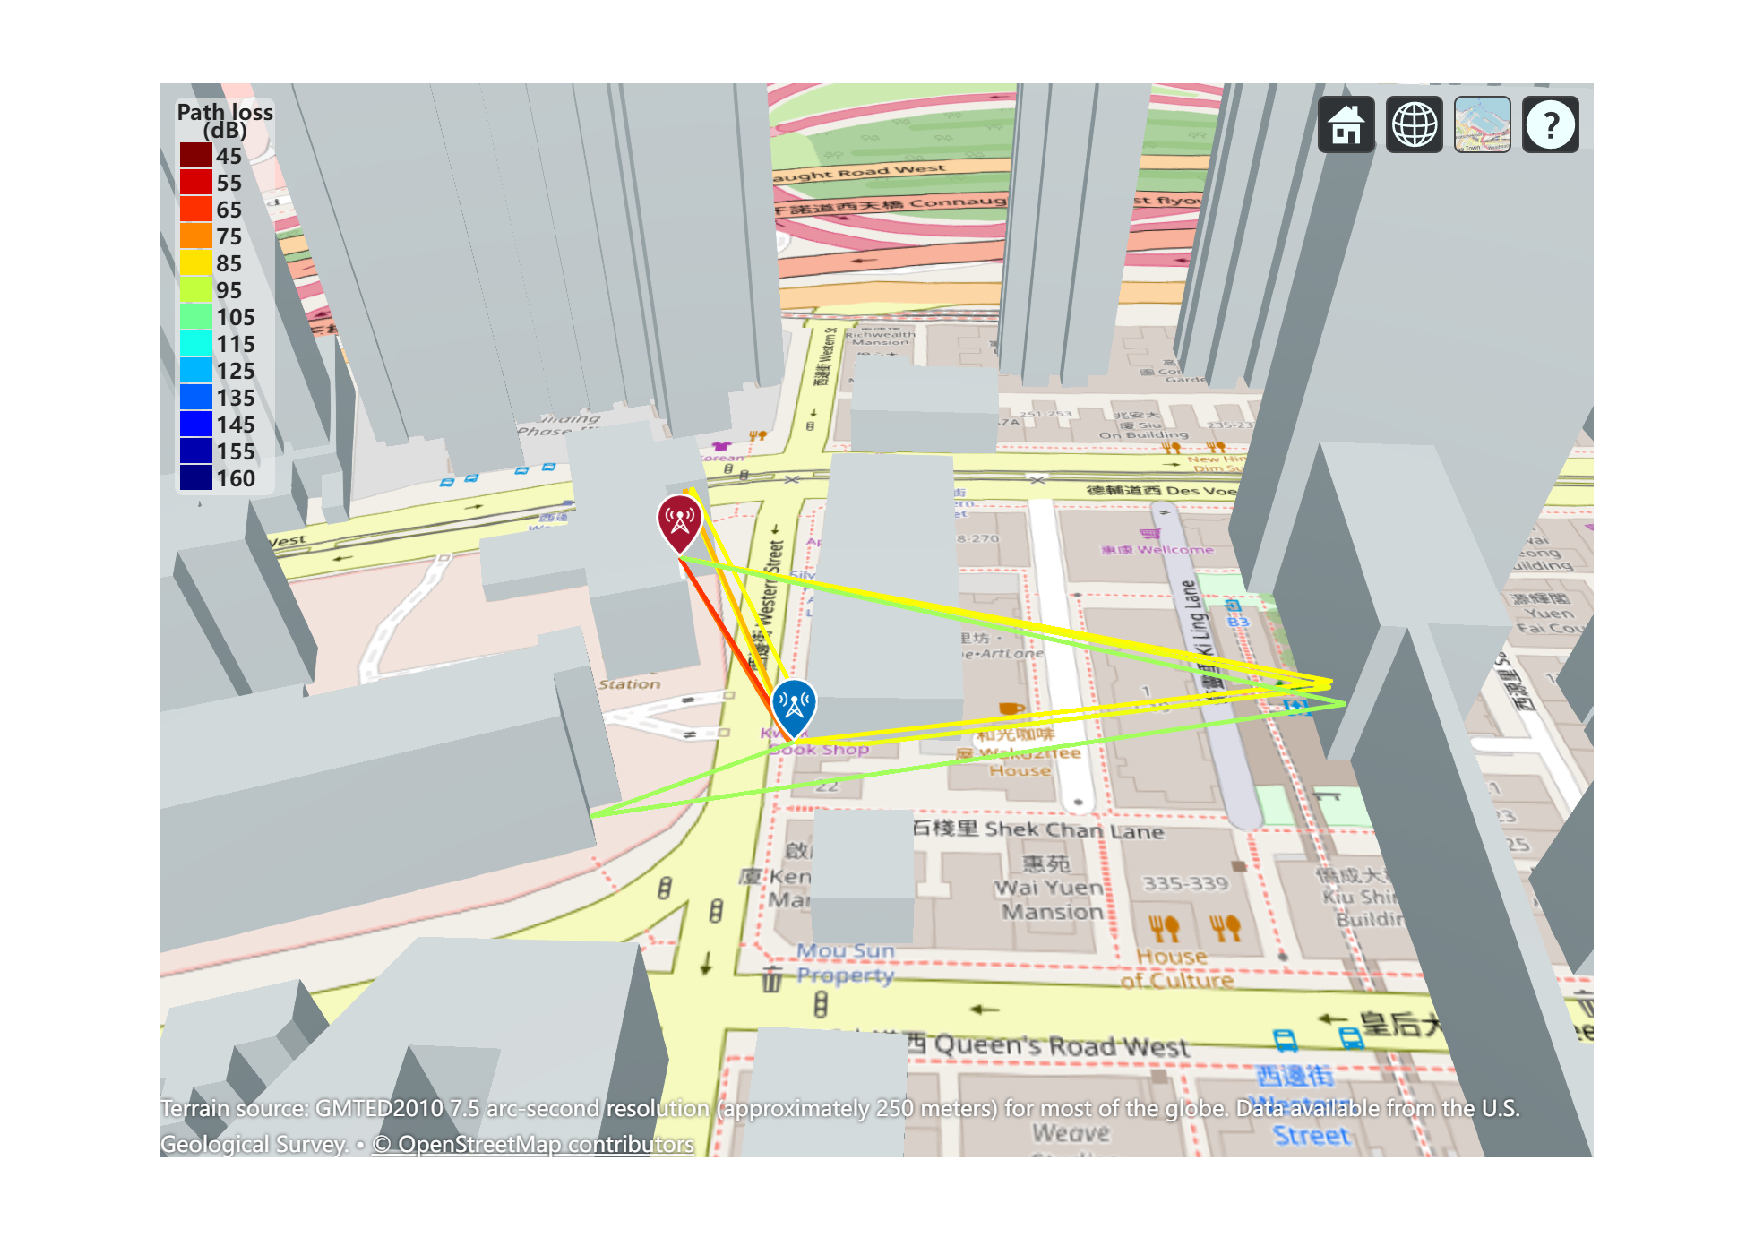
\includegraphics[width=0.5\textwidth]{figs/ray_tracing.pdf} 
		\caption{\color{red}The model built from ray tracing scheme in Matlab, which is based on buildings in Hong Kong.} 
		\label{fig_ray_tracing}
	\end{figure}
	
	\begin{figure}[H]
		\centering 
		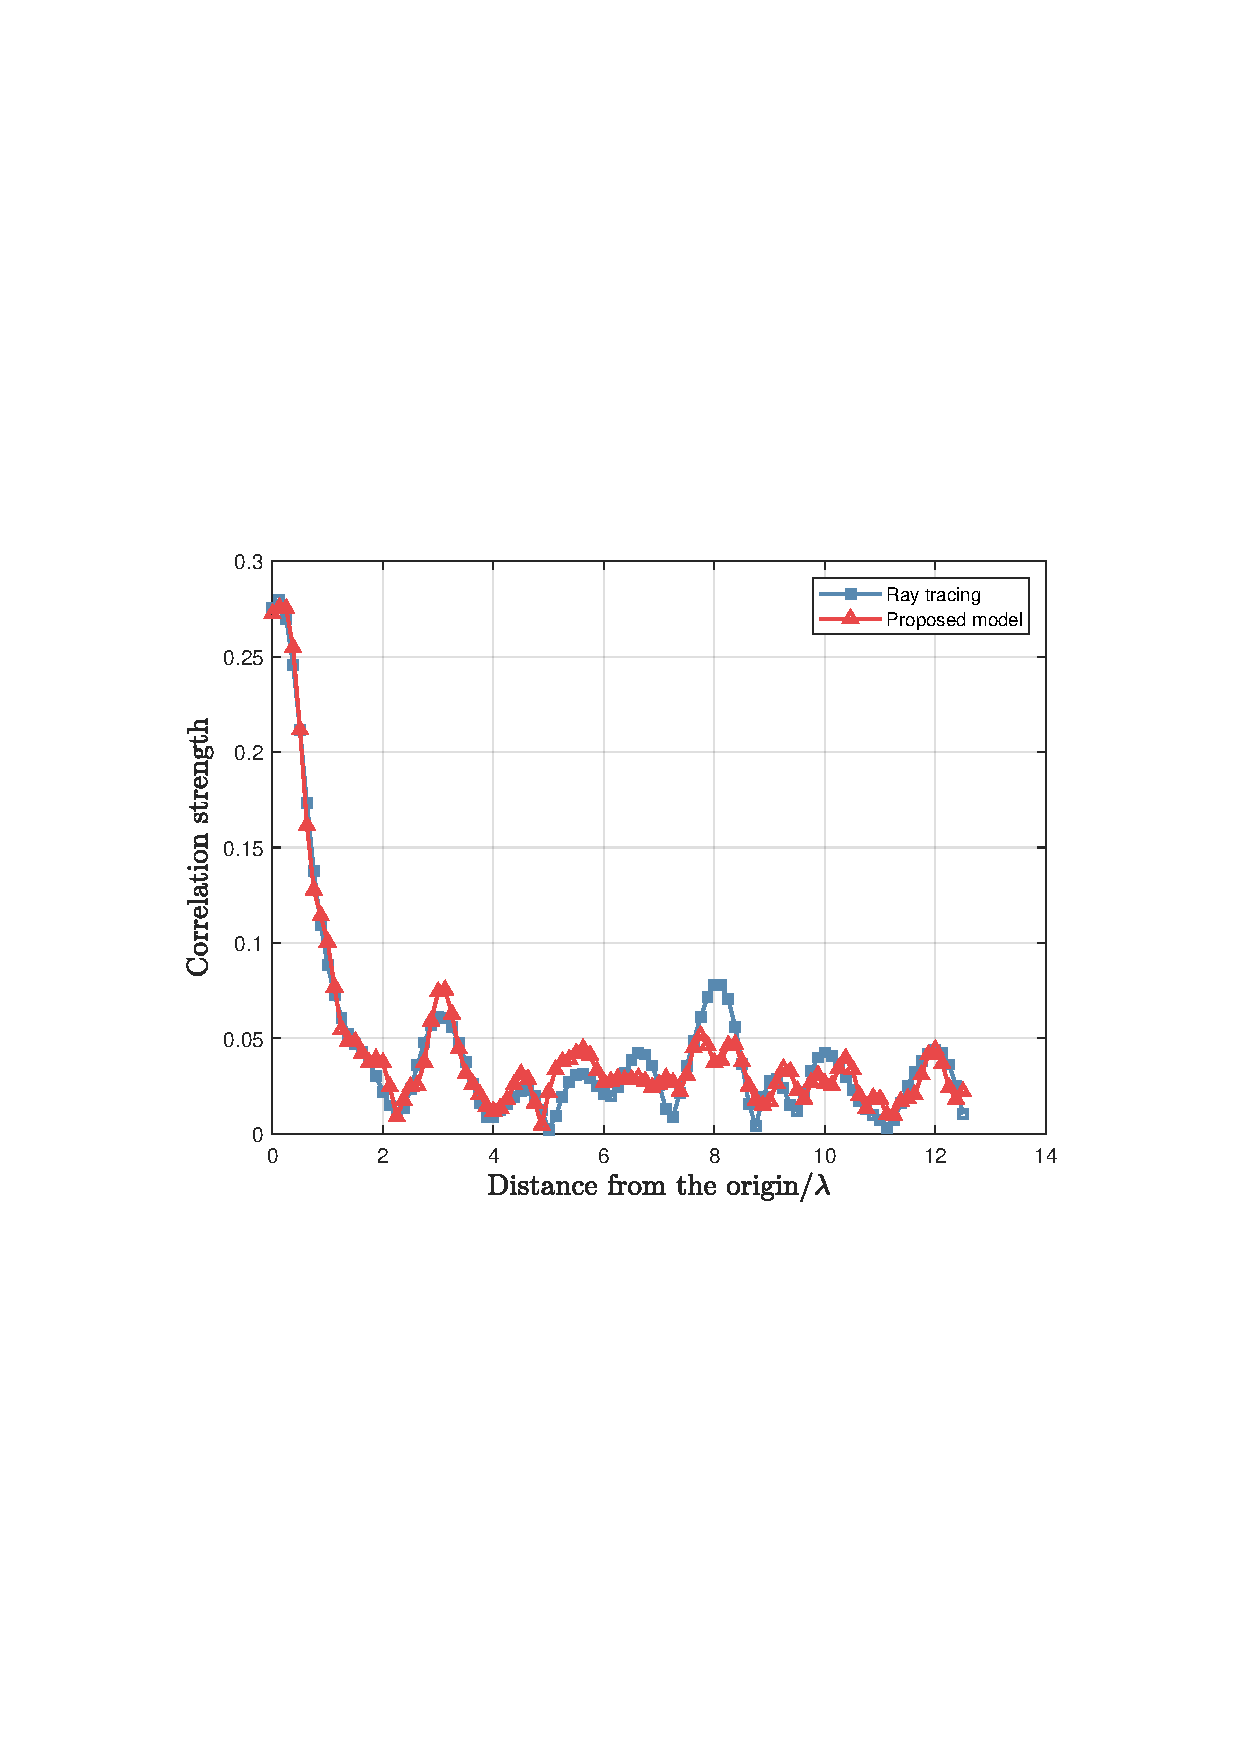
\includegraphics[width=0.5\textwidth]{figs/ray_tracing_fit_one_side.pdf} 
		\caption{\color{red}Comparison between the proposed model and the model built from ray tracing scheme.} 
		\label{fig_ray_tracing_fit}
	\end{figure}

\end{framed}

\textbf{Reviewer 3:}
As a second step, the authors show the sparsity of the proposed channel model by observing the received signal in the wave domain. However, the sparsity of the channel is not a characteristic of the model but rather a characteristic of the propagation in relation to the considered scenario the model wants to capture, particularly the number of scatterers. It is well-known that in the presence of three scatterer regions, as considered in Fig. 8, the channel seen in the wave domain results in sparsity. I do not see anything new here. If one considers more scatterers, then the channel becomes less sparse. Moreover, the analysis of extended scattered regions in the wave domain can be found in the textbook "Wave Theory of Information" by Franceschetti.

{\color{blue}{\textbf{Authors: } 
Thanks for the reviewer for pointing out this problem. We agree with the reviewer that the sparsity is the characteristic of the channel, not the proposed model. We have reorganized the corresponding part in the paper, not emphasizing the sparsity as the contribution. 
We plot the wavenumber domain of the model for two reasons:
1. it can help to construct the approximate correlation function according to the received noisy field, so as to provide electromagnetic prior information for channel estimation and improve the channel estimation equality. 
We explain this in the paper as follows:
}}

\begin{framed}
	{\bf Section IV.C}

	\quad {\color{red}If the channel is sparse, from the law of large numbers, we know that $h$ has power peaks in wavenumber domain,
	which can be used in channel estimation of reconstruction procedure to improve the accuracy.} Specifically, if we reshape the vector ${\bf h}$ to a matrix ${\bf H}_{i,:} = {\bf h}_{(i-1)*N_z+1:i*N_z,1}^{\rm T}$, its sparsity in wavenumber domain can be expressed as follows:
	\begin{equation}
		\begin{aligned}
			{\mathbb E}[\left|({\bf F}_1{\bf H}{\bf F}_2)_{i,j}\right|^2] &= {\mathbb E}\left[ \left| \sum_{i'}\sum_{j'}{\bf F}_{1,i,j'}{\bf H}_{i',j'}{\bf F}_{2,i',j}^{\rm H} \right|^2 \right]
			\\& ={\mathbb E}\left[ \sum_{i'_1,i'_2,j'_1,j'_2}{\bf F}_{1,i,j'_1}{\bf H}_{i'_1,j'_1}{\bf F}_{2,i'_1,j}^{\rm H}{\bf F}^{*}_{1,i,j'_2}{\bf H}^{*}_{i'_2,j'_2}{\bf F}_{2,i'_2,j}^{\rm T}\right]
			\\& = \sum_{i_1',i_2',j'_1,j'_2} e^{{\rm j}\frac{2k}{N_y-1}(i-\frac{N_y+1}{2})(j_1'-j_2')d_y}R({\bf r}_1,{\bf r}_2)
			e^{{\rm j}\frac{2k}{N_z-1}(j-\frac{N_z+1}{2})(i_2'-i_1')d_z},
		\end{aligned}
		\tag{23}
	\end{equation}
\end{framed}

{\color{blue}
2. the wavenumber domain of the model has relationship to the channel DoF from the spatial bandwidth perspective. We add the explanation of it in the paper:
}

\begin{framed}
	{\bf Section IV.C}

	\quad For the near-field scattering scenario, the scattering region will correspond to an area rather than a point in the wavenumber domain. The shape of the area reflects the size, directions and concentration parameters of the scattering region. {\color{red} It is also worth noting that the area relates to the concept called spatial bandwidth [13]. The larger the area is, the larger the spatial bandwidth is, which provides more possible DoF for the wireless communication system. Further discussion about the DoF will be presented in the following subsection.}
\end{framed}

{\color{blue}
We also agree with the reviewer that the wavenumber sparsity itself does not have enough novelty. To strengthen the contribution of the paper, we add an extra part, which follows point 2 to discuss the DoF under the proposed channel model. Specifically, we first ultilize spatial bandwidth in [13] and then further analyze the DoF based on conclusions in [43]. Detailed revisions are shown in the following box:
}

\begin{framed}
    {\bf{Section IV.D \color{red}Channel DoF of the proposed model}}

	\setcounter{equation}{23}
	\setcounter{figure}{9}

    \quad In this section we will discuss how the parameters influence the performance of the system from the degree of freedom (DoF) perspective.
    The DoF of the channel depends on the eigenvalue distribution of the model. If the eigenvalue decay rate is slow, there exist multiple subchannels that can support communication at a certain rate, leading to greater DoF. On the contrary, if few eigenvalues are obviously larger than other eigenvalues, the DoF will be small [21]. 
    
    \quad {\color{red} We will provide some insights of the DoF from the spatial bandwidth [13] perspective and then verify them by numerical analysis of the proposed model. The spatial bandwidth characterizes the band-limiting effect of electromagnetic fields in the wavenumber domain, which is similar to the classical bandwidth that depicts a function's band-limiting effect in the frequency domain. The spatial bandwidth shows the electromagnetic fields' DoF through spatial sampling. In [13], the scattered electromagnetic waves ${\bf E}({\bf r})$ are observed on an infinite line or region at the receiver. In this paper we adopt scalar form of the electromagnetic field, leading to $E({\bf r}) = \int_{V} g({\bf r},{\bf r}')(k^2({\bf r}')-k_0^2)  E({\bf r}'){\rm d}{\bf r}'$. We have $\bar{E}({\bf r}) = E({\bf r})e^{-{\rm j}k_0\left\|{\bf r} \right\|}$ to single out the phase factor introduced by the distance, and $X({\bf r}) = (k^2({\bf r})-k_0^2)  E({\bf r})$ on the scatterer surface. Then we have
    \begin{equation}
        \bar{E}({\bf r}) = \int_V \bar{g}({\bf r},{\bf r}') X({\bf r}') {\rm d}{\bf r}',
    \end{equation}
    where $\bar{g}({\bf r},{\bf r}') = \frac{1}{2\pi}\frac{e^{{\rm j}k_0(\left\| {\bf r}-{\bf r}' \right\|-\left\| {\bf r} \right\|)}}{\left\| {\bf r}-{\bf r}' \right\|}$. For simplicity, we focus on the one-dimensional receiver and abbreviate $\bar{E}({\bf r})$ as $\bar{E}({r})$, $\bar{g}({\bf r},{\bf r}')$ as $\bar{g}({r},{\bf r}')$, where $r$ is along a chosen line determined by ${\bf r}$ in the three-dimensional space. To show the how $\bar{E}({r})$ is band-limited in the wavenumber domain, we introduce $\bar{E}_w({r}) = \bar{E}({r}) * \frac{\sin w r}{r}$ which performs low-pass filtering on $\mathscr{F}[\bar{E}({r})]$. Then we have 
    \begin{equation}
        \bar{E}_w({r}) = \int_V \bar{g}_w({r},{\bf r}') X({\bf r}') {\rm d}{\bf r}',
    \end{equation}
    where 
    \begin{equation}
        \begin{aligned}
        \bar{g}_w({r},{\bf r}') &= \frac{1}{2\pi^2} \int_{-\infty}^{+\infty} \frac{\sin w(r-\xi)}{r-\xi}\frac{e^{{\rm j}k_0(\left\| \boldsymbol{\xi}-{\bf r}' \right\|-\left\| \boldsymbol{\xi} \right\|)}}{\left\| \boldsymbol{\xi}-{\bf r}' \right\|}{\rm d}\xi
        \\& \overset{a}{=} \frac{1}{2\pi^2{\rm j}} \int_{C^+} \frac{e^{ {\rm j}w(r-\xi)}}{r-\xi}\frac{e^{{\rm j}k_0(\left\| \boldsymbol{\xi}-{\bf r}' \right\|-\left\| \boldsymbol{\xi} \right\|)}}{\left\| \boldsymbol{\xi}-{\bf r}' \right\|}{\rm d}\xi 
        \\& ~~~~- \frac{1}{2\pi^2{\rm j}} \int_{C^-} \frac{e^{ -{\rm j}w(r-\xi)}}{r-\xi}\frac{e^{{\rm j}k_0(\left\| \boldsymbol{\xi}-{\bf r}' \right\|-\left\| \boldsymbol{\xi} \right\|)}}{\left\| \boldsymbol{\xi}-{\bf r}' \right\|}{\rm d}\xi 
        \\&~~~~+ \bar{g}({r},{\bf r}'),
        \end{aligned}
    \end{equation}
    in which $\overset{a}{=}$ is from the residual theorem, $C^+$ and $C^-$ are two paths above and below the real axis.
    The spatial bandwidth is the minimum $w$ that makes $\left\|\bar{E}(r)-\bar{E}_w(r)\right\|$ small enough. 
    We have 
    \begin{equation}
        \begin{aligned}
        \left\|\bar{E}(r)-\bar{E}_w(r)\right\| &=  \left[\int_{-\infty}^{+\infty}  \left|\bar{E}(r)-\bar{E}_w(r)\right|^2{\rm d}r \right]^{\frac{1}{2}}
        \\& \leqslant \underset{{\bf r}'}{\rm max} \left[ \int_{-\infty}^{+\infty} \left| \Delta \bar{g}({r},{\bf r}') \right|^2{\rm d}{\bf r}'  \right]^{\frac{1}{2}} 
        \\& ~~~~\cdot \int_V \left| X({\bf r}') \right| {\rm d}{\bf r}',
        \end{aligned}
    \end{equation}
    where $\Delta \bar{g} = \bar{g}-\bar{g}_w$ is the item corresponds to the spatial bandwidth $w$. We can further express it by
    \begin{equation}
        \begin{aligned}
            \Delta \bar{g}({r},{\bf r}')& =  \frac{1}{2\pi^2{\rm j}} \int_{C^+} \frac{e^{ {\rm j}w(r-\xi)}}{r-\xi}\frac{e^{{\rm j}k_0(\left\| \boldsymbol{\xi}-{\bf r}' \right\|-\left\| \boldsymbol{\xi} \right\|)}}{\left\| \boldsymbol{\xi}-{\bf r}' \right\|}{\rm d}\xi 
            \\& ~~~~- \frac{1}{2\pi^2{\rm j}} \int_{C^-} \frac{e^{ -{\rm j}w(r-\xi)}}{r-\xi}\frac{e^{{\rm j}k_0(\left\| \boldsymbol{\xi}-{\bf r}' \right\|-\left\| \boldsymbol{\xi} \right\|)}}{\left\| \boldsymbol{\xi}-{\bf r}' \right\|}{\rm d}\xi. 
        \end{aligned}
    \end{equation}
    The following part is similar to [13], which shows that when $w>{\rm max}\frac{\partial \left( k_0\left( \left\| \boldsymbol{\xi}-{\bf r}' \right\|-\left\| \boldsymbol{\xi} \right\| \right) \right)}{\partial \xi}$, $\Delta \bar{g}$ converges to 0 faster than any power. Moreover, when $w<{\rm max}\frac{\partial \left( k_0\left( \left\| \boldsymbol{\xi}-{\bf r}' \right\|-\left\| \boldsymbol{\xi} \right\| \right) \right)}{\partial \xi}$, $\Delta \bar{g}\approx \bar{g}$. Therefore, $w_0 = {\rm max}\frac{\partial \left( k_0\left( \left\| \boldsymbol{\xi}-{\bf r}' \right\|-\left\| \boldsymbol{\xi} \right\| \right) \right)}{\partial \xi}$ can be chosen as the spatial bandwidth of the received electromagnetic field. From geometrical analysis, it is easy to find that the maximum of $\frac{\partial \left( k_0\left( \left\| \boldsymbol{\xi}-{\bf r}' \right\|-\left\| \boldsymbol{\xi} \right\| \right) \right)}{\partial \xi}$ only depends on the radius $r_s$ of the scatterer, and the inner structure of the scatterer does not have obvious influence on the DoF. Moreover, we can bound $w_0$ by $\frac{2\pi r_s}{\lambda}<w_0<\sqrt{2}\frac{2\pi r_s}{\lambda}$, where $r_s$ is the radius of the scatterer. The lower bound of $w_0$ is achieved when $\boldsymbol{\hat{\mu}} = \boldsymbol{\hat{\mu}}_0$ satisfies the condition that the corresponding scatterer surface is tangent to $OF$, as shown in Fig. \ref{fig_mu}. When $\boldsymbol{\hat{\mu}} \neq \boldsymbol{\hat{\mu}}_0$, the lower bound of $w_0$ will be less than $\frac{2\pi r_s}{\lambda}$. Specifically, we can obtain 
\begin{equation}
	\begin{aligned}
		w_0&>\frac{2\pi d }{\lambda} 2\sin \frac{\alpha}{2} \cos \frac{\alpha}{2} = \frac{2\pi d \sin \alpha}{\lambda}
		\\& = \frac{2\pi d}{\lambda} \frac{r_s \cos(\alpha_0+\theta)}{\sqrt{(d-r_s\sin(\alpha_0+\theta))^2+(r_s\cos(\alpha_0+\theta))^2}}
		\\& = \frac{2\pi d}{\lambda}\frac{r_s\cos(\alpha_0+\theta)}{\sqrt{d^2+r_s^2-2dr_s\sin(\alpha_0+\theta)}},
	\end{aligned}
\end{equation}
}{\textcolor{red}{
where $\sin(\alpha_0)=\frac{r_s}{d}$ and $\cos(\theta) = \boldsymbol{\hat{\mu}}\cdot\boldsymbol{\hat{\mu}}_0 $.}
}

\begin{figure}[H]
	\centering 
	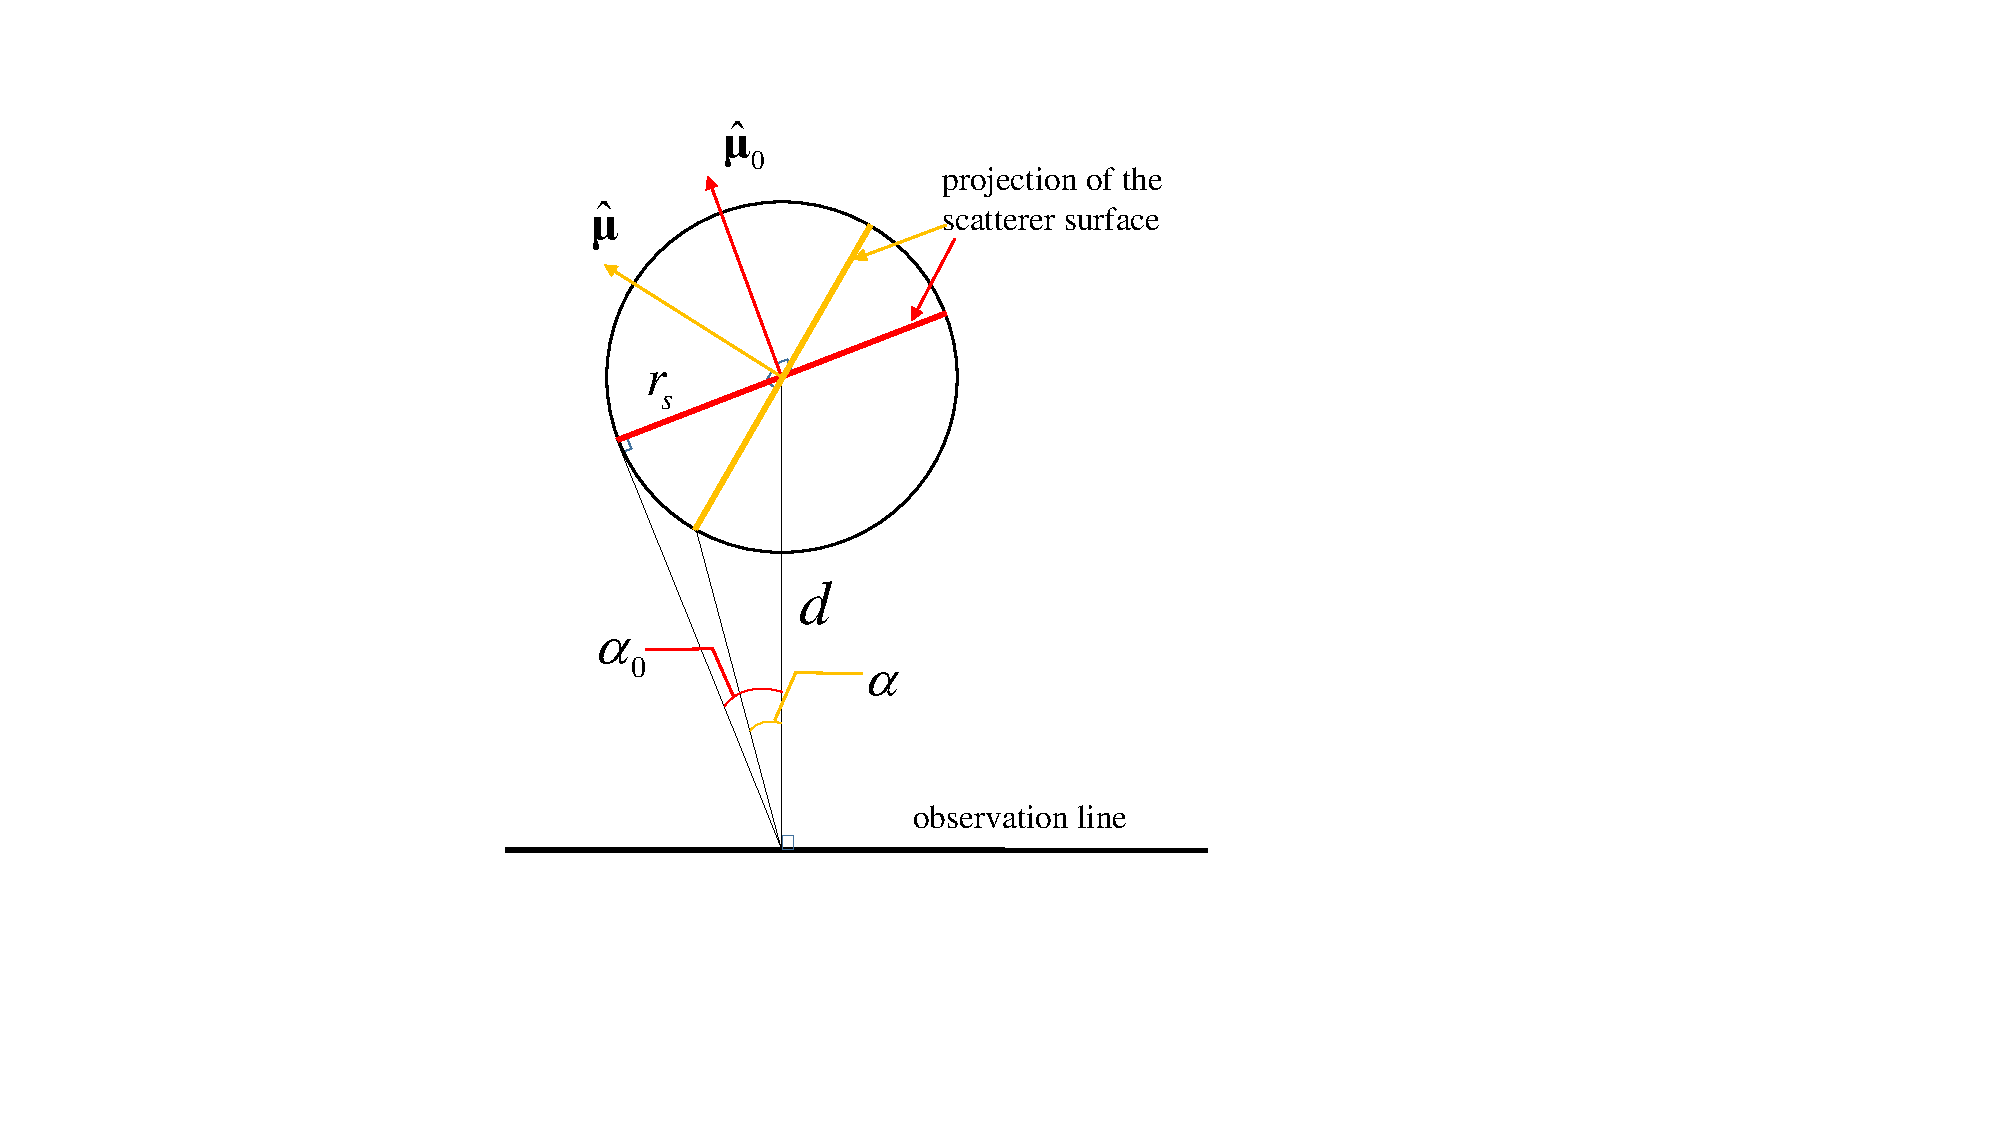
\includegraphics[width=0.5\textwidth]{figs/dof_consider_mu.pdf} 
	\caption{\color{red}Concerning the spatial bandwidth with respect to different $\boldsymbol{\hat{\mu}}$.} 
	\label{fig_mu}
\end{figure}

{\textcolor{red}{
From the above analysis we know that the spatial bandwidth and channel DoF mainly rely on the outermost layer of the scattering region. To be more specific, smaller $r_s$ leads to smaller scattering regions, which reduces the DoF. When $a$ is smaller than $0$, the scattering region can be viewed as the outermost circle combined with the inner part, and the DoF will not change heavily with $a$. When all the scattering power comes from the outermost circle, which plays the most important role in affecting the DoF, the DoF will be the largest. Therefore, the DoF reaches the maximum when $a$ approaches $-1$. For two-dimensional receiver adopted in this paper, we can decompose the surface in two different directions, each with spatial bandwidth $w_0$.}
}
    
{\color{red}
    \quad Then, we plot the eigenvalues of the correlation matrix when the radius and shape of the scattering region vary in Fig. \ref{fig_eigen_a} and Fig. \ref{fig_eigen_r}. We can observe that the DoF of the channel will increase with the radius $r$ of the scatterer, and decrease when $a$ increases. When $a$ approximates $-1$, which corresponds to the case that the scatterer tends to a ring, the DoF of the channel reaches the maximum, which coinsides with the spatial bandwidth analysis.
    
    \quad Note that the spatial bandwidth analysis is based on the infinitely large observation region of the received electromagnetic fields. For practical scenarios with limited observation region, the observed field can not be strictly band-limited in the wavenumber domain. Moreover, the spatial sampling period should not be equal to that in sampling theorem because the points far away from the scatterer are not as important as the ones close to the scatterer. This problem is discussed in [43] and the tool of cut-set integral is introduced. Results of the approximated DoF considering a closed surface as the receiver that encloses the source are discussed in [43], which we will follow to provide DoF bounds in the scenario with square receiving surface. 
    
    \quad Here we discuss a simple scenario that the line between the center of the scatterer and the center of the receiving surface is vertical to the receiving surface. We construct two spheres concentric with the scatterer region. These spheres satisfy the condition that the receiving surface is inscribed in a circle $C_1$ on the large sphere $S_1$, and its four sides are externally-tangent to a circle $C_2$ on the small sphere $S_2$, as shown in Fig. \ref{fig_circles}. We denote the two spherical caps of $S_1$ divided by $C_1$ as $S'_1$ and $S''_1$, where $S'_1$ is the larger one. Similarly we have $S'_2$ and $S''_2$. Since the information flows through any closed surface that encloses the scatterer should be the same, we know that the electromagnetic fields on $C_1$ and $S''_1$ have the same DoF, so as $C_2$ and $S''_2$. According to [43] we know that the DoF on the sphere $S_1$ and $S_2$ are $N_0 = O(r_s^2/\lambda^2)$.} {\color{red}From symmetry on the sphere\footnote{\color{red}Here the asymmetry introduced by $\hat{\boldsymbol{\mu}}$ is not considered since it is hard to evaluate. By considering this asymmetry a more accurate result will be obtained.} and simple geometry, the DoF $N_1$ on $S''_1$ can be expressed by
    \begin{equation}
        N_1 \approx N_0\frac{\mathcal{A}_{S''_1}}{\mathcal{A}_{S_1}}= N_0\frac{2\pi\sqrt{d^2+r_m^2}(\sqrt{d^2+r_m^2}-d)}{4\pi(d^2+r_m^2)}.
    \end{equation}
    Similarly we know that the DoF $N_1$ on $S''_1$ can be expressed by $N_2 \approx N_0 \frac{2\pi\sqrt{2d^2+r_m^2}(\sqrt{2d^2+r_m^2}-\sqrt{2}d)}{4\pi(2d^2+r_m^2)}$.
    Then we have $N_2\leqslant N_{\rm receiver} \leqslant N_1$. Note that when $d\gg r_m$, both $N_1$ and $N_2$ approximates $O(\frac{r_s^2r_m^2}{\lambda^2d^2})$, which coincides with [44]. On the contrary, if $r_m \gg d$, $N_{\rm receiver} \approx \frac{N_0}{2}$, because it can be viewed as an infinitely-large surface which gets half of the overall electromagnetic waves out of the scatterer. Under this scenario the DoF has little relationship with the distance between the scatterer and the receiver, which coincides with [13]. Here the asymmetry introduced by $\hat{\boldsymbol{\mu}}$ is not considered since it is hard to evaluate. By considering this asymmetry a more accurate result will be obtained.
    }
    
    \begin{figure}[H]
          \centering 
          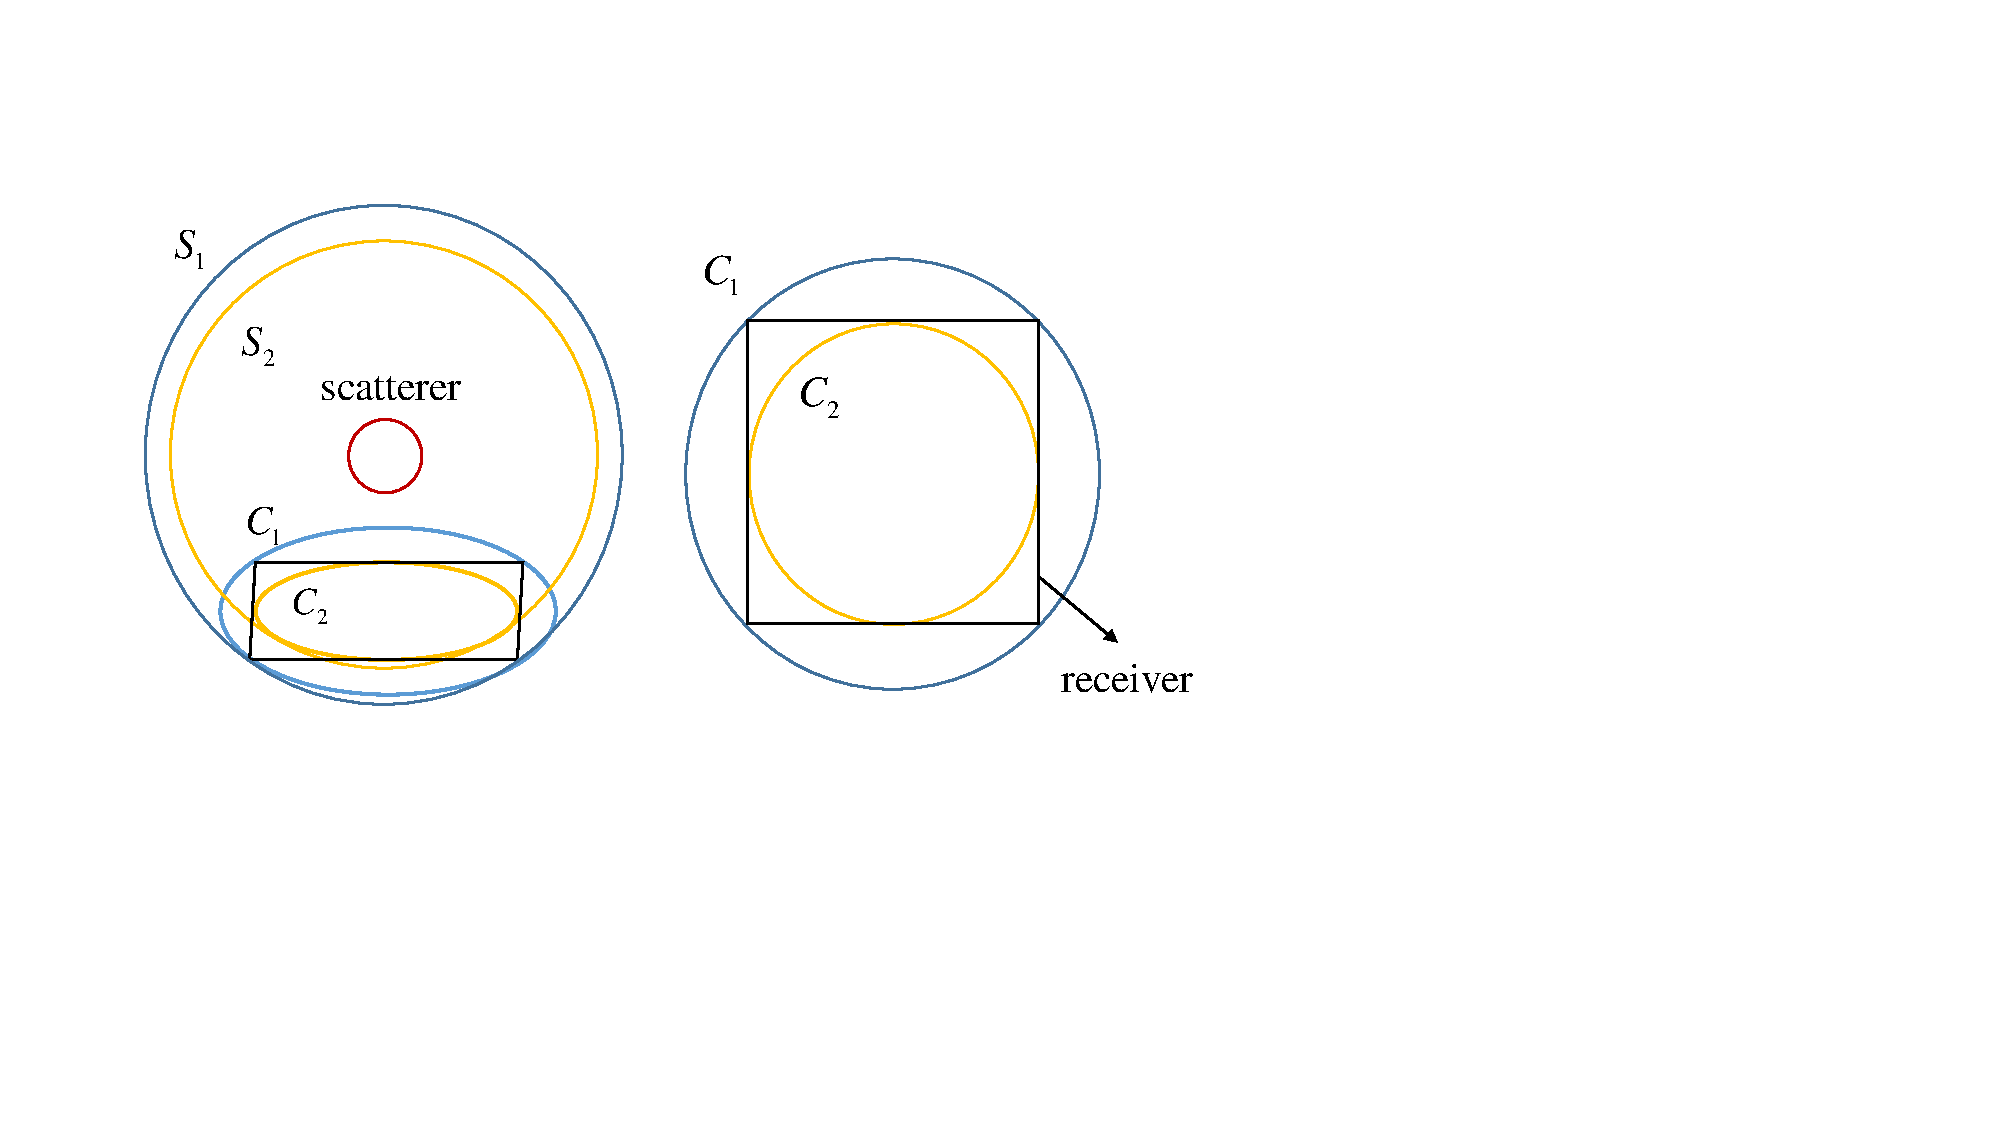
\includegraphics[width=0.6\textwidth]{figs/circles.pdf} 
          \caption{\color{red}The receiving surface that is inscribed in $C_1$ and externally-tangent to $C_2$, where $C_1$ and $C_2$ are on $S_1$ and $S_2$ separately.} 
          \label{fig_circles}
      \end{figure}
    
    

    \begin{figure}[H]
        \centering 
        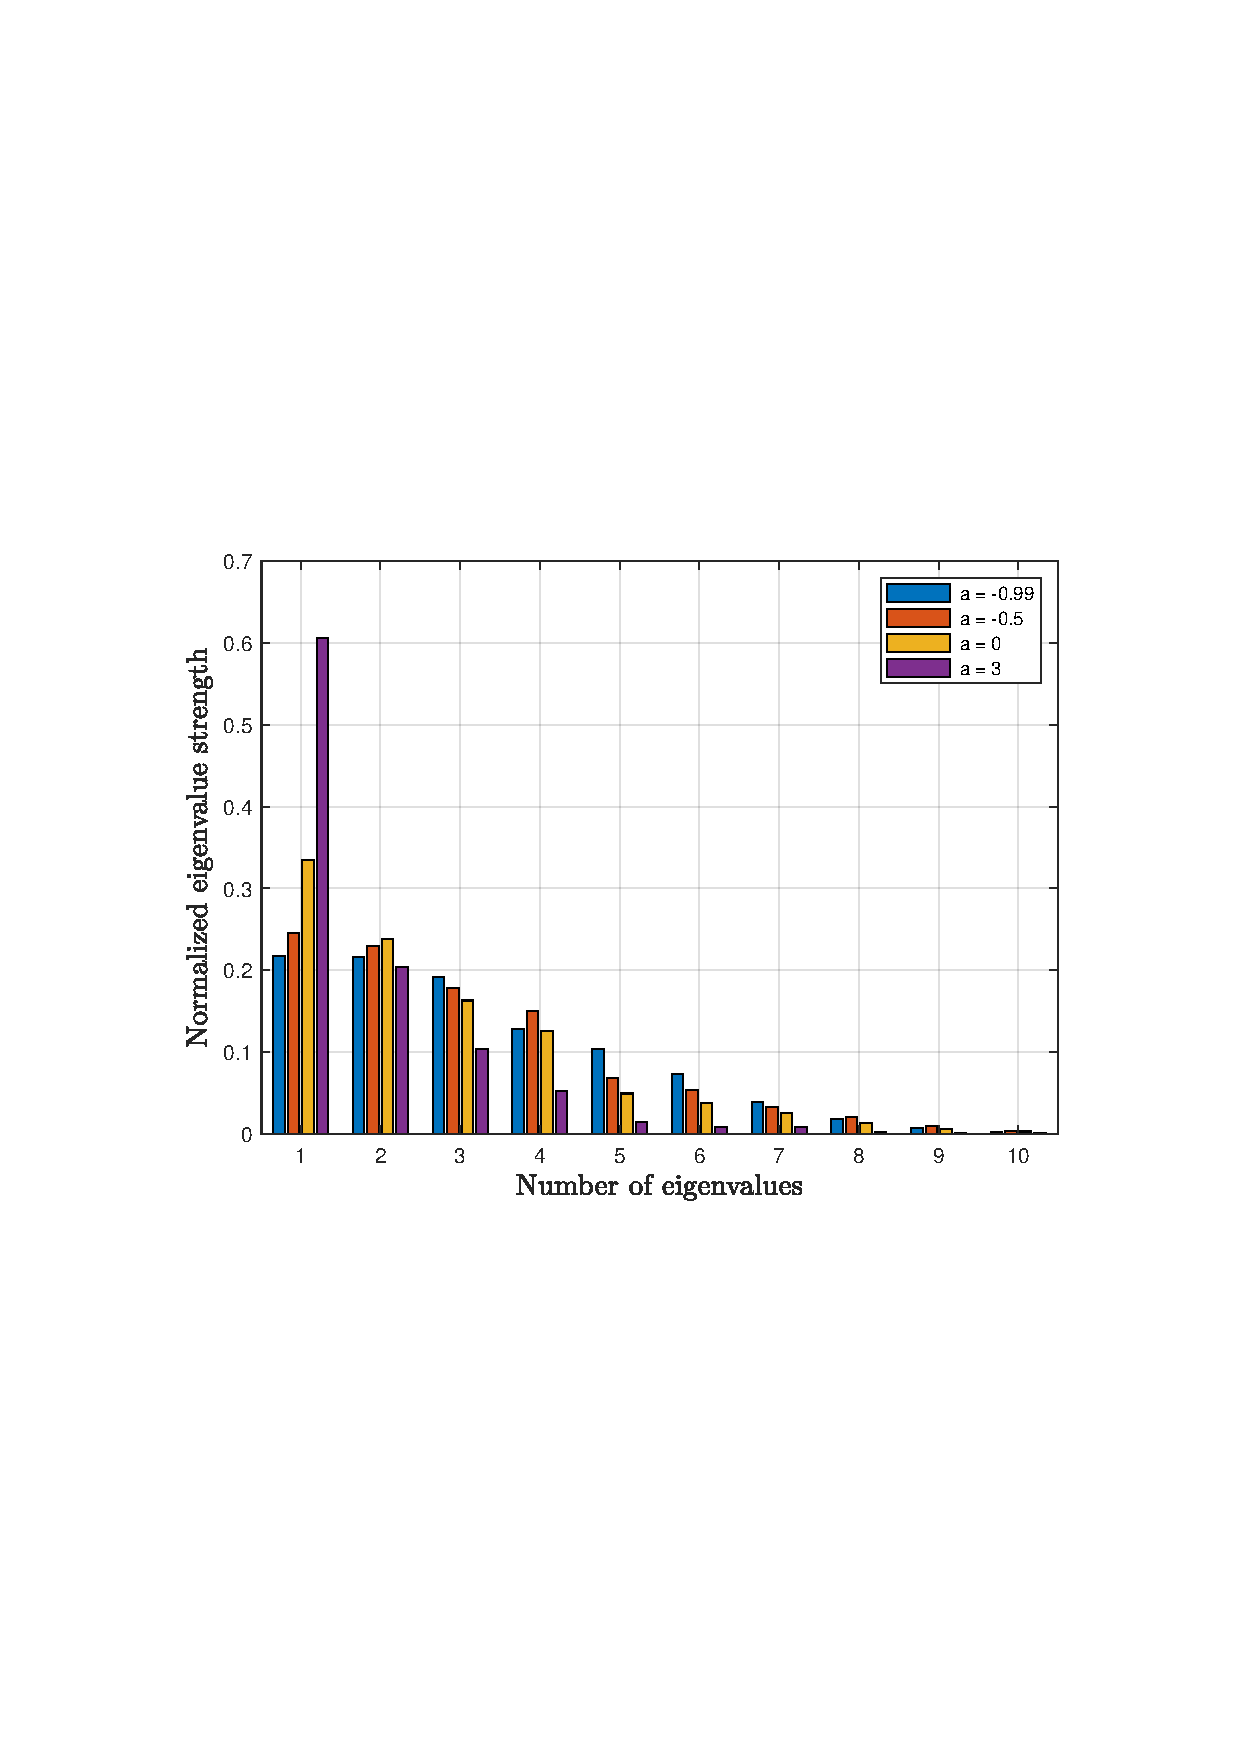
\includegraphics[width=0.5\textwidth]{figs/eigen_a.pdf} 
        \caption{The eigenvalues of the correlation matrix in decreasing order with ${\bf d}$ fixed to $[-100,100,-100]\,{\rm m}$, $\boldsymbol{\mu}$ fixed to $[-\frac{1}{\sqrt{3}},\frac{1}{\sqrt{3}},-\frac{1}{\sqrt{3}}]$, and $r=5\,{\rm m}$. The concentration parameter $a$ varies.} 
        \label{fig_eigen_a}
    \end{figure}
    \begin{figure}[H]
        \centering 
        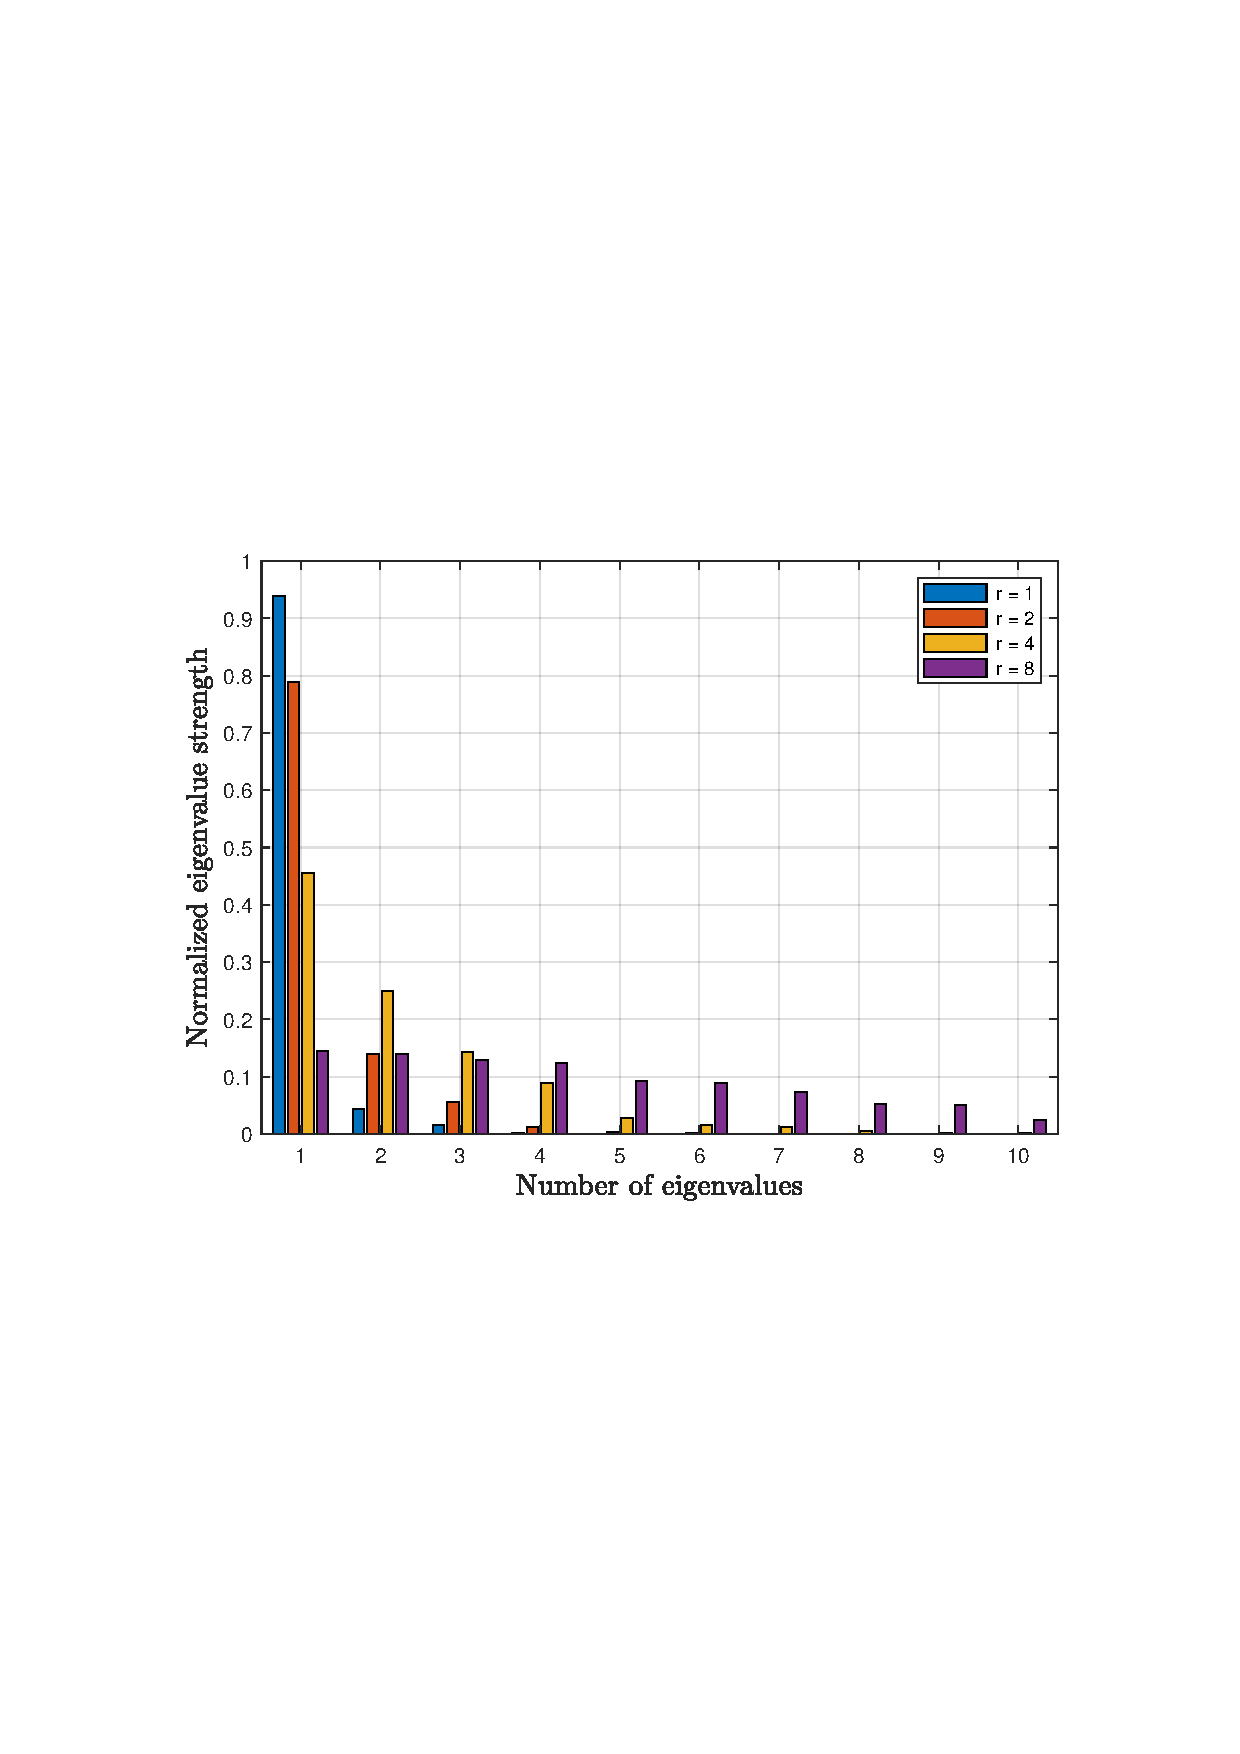
\includegraphics[width=0.5\textwidth]{figs/eigen_r.pdf} 
        \caption{The eigenvalues of the correlation matrix in decreasing order with ${\bf d}$ fixed to $[-100,100,-100]\,{\rm m}$, $\boldsymbol{\mu}$ fixed to $[-\frac{1}{\sqrt{3}},\frac{1}{\sqrt{3}},-\frac{1}{\sqrt{3}}]$, and $a=0$. The radius $r$ varies.} 
        \label{fig_eigen_r}
    \end{figure}
    
\end{framed}

\textbf{Reviewer 3:}
Finally, the proposed channel estimation algorithm is interesting but, contrary to what is stated, it is not based on the proposed model but only on the consideration that the channel is in the near field and sparse. In fact, nothing from the proposed model is used in the estimator. In fact, it has also been validated using the classical 3GPP CDL model. I would see this section as a contribution to submit in a separate paper.

{\color{blue}{\textbf{Authors: } 
Thanks for the reviewer's valuable comments. The proposed model is used in the channel estimator to construct an approximate channel correlation function when the sparsity of the channel in the wavenumber domain is obtained. It can be viewed as an improvement method compared to [24], which construct the channel correlation function from isotropic incident waves. We add the explanation about the relationship between the channel estimation scheme and the proposed model. Detailed revisions are shown in the following box: 
}}

\begin{framed}
	{\bf{Section V}}

	\quad After discussing the properties of the analytical channel model, we will propose a near-field channel estimation scheme based on the model. {\textcolor{red}{We first perform Fourier transformation on the observed field to capture the power peaks in the wavenumber domain. Then we use the }{\color{red} proposed model, which provides the prior information of electromagnetic fields, to reconstruct an approximate channel correlation function. This approach is similar to the subspace based channel estimation scheme in [24], which constructs the correlation function based on isotropic scattering field. Compared to [24], our scheme provides more prior information of electromagnetic fields of the fields by using the proposed channel model. Therefore, it can achieve better performance than the existing schemes. }}In the channel estimation procedure, the received field is denoted by ${\bf y}=\sqrt{P}{\bf h}+{\bf n}$, where $P$ is the signal-to-noise ratio, ${\bf h}$ is generated from the channel coupling matrix, and ${\bf n} \sim \mathcal{CN}(0,{\bf I})$ is the noise vector. 
\end{framed}


\textbf{Reviewer 3:}
Minor comments:

After Eqn. (5): What is $\hat{\mu}$?

{\color{blue}{\textbf{Authors: } 
Thanks for the reviewer's valuable comments. Since the scattering region, as assumed in the paper, is a circular surface. It should have a certain direction, which we represent as $\boldsymbol{\hat{\mu}}$. Specifically, it is the direction that is tangent to the scatterer surface.

 Detailed revisions are shown in the following box: 
}}

\begin{framed}
	{\bf{Section III.A}}

	\quad We further assume that the scattering region $V$ is distributed in a solid circle, centering at ${\bf d}$ and perpendicular to $\hat{\boldsymbol{\mu}}$, which means that $\hat{\boldsymbol{\mu}}^{\rm T}({\bf r}'-{\bf d})=0 $. {\color{red}Here $\hat{\boldsymbol{\mu}}$ represents the direction of the scattering surface.}
\end{framed}

{\color{blue}
The meaning of $\boldsymbol{\hat{\mu}}$ is also shown in Fig. 1, as 
\begin{figure}[H]
	\centering 
	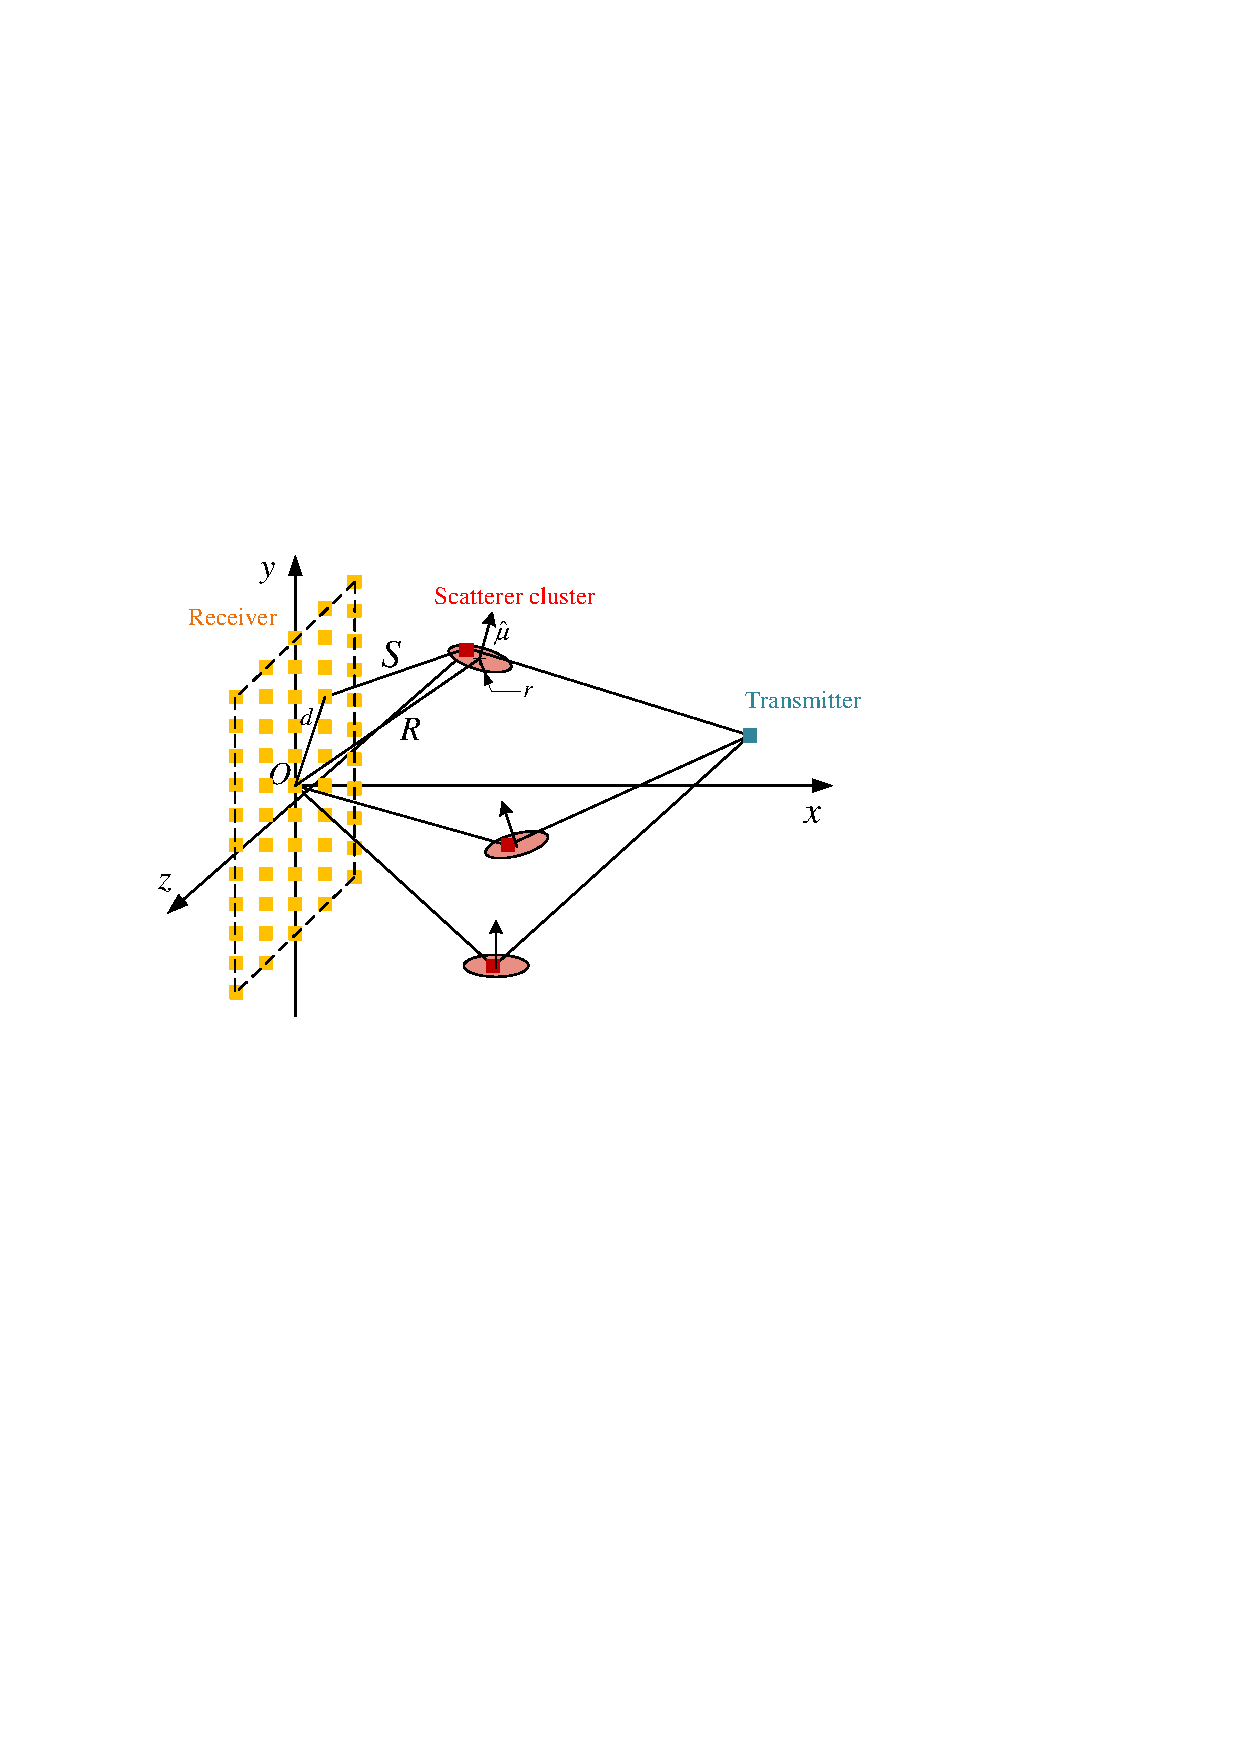
\includegraphics[width=0.5\textwidth]{figs/threedimension_solid_circle.pdf} 
	\label{fig_3d_solid_sphere}
\end{figure}
}

\textbf{Reviewer 3:}
The autocorrelation function is initially named $R_E(r_1,r_2)$, then $R(r_1,r_2)$. Please, adopt the same symbol.

{\color{blue}{\textbf{Authors: } 
Thanks to the reviewer for pointing out this problem. We have add explanations in the paper, clarifying that we use $R$ instead of $R_E$ for simplicity. Then we replace the rest of the $R_E$ with $R$. Detailed revisions are shown in the following box:
}}

\begin{framed}
	{\bf{Section III.A}}

	\quad By omitting the first item in (\ref{equ_scattering_field}) which represents the deterministic line-of-sight component, we have 
\begin{equation}
	\begin{aligned}
	R_E({\bf r}_1,{\bf r}_2) =& \mathbb{E} \Big[\int_V\int_V g({\bf r}_1,{\bf r}_1')g^{*}({\bf r}_2,{\bf r}_2')(k^2({\bf r}'_1)-k_0^2)
	\\& (k^2({\bf r}'_2)-k_0^2) E({\bf r}_1') E^{*}({\bf r}_2') {\rm d}{\bf r}_1'{\rm d}{\bf r}_2'\Big],
	\end{aligned}
	\tag{8}
	\label{equ_correlation_complicated}
\end{equation}
{\color{red}where in the rest part of the paper we express $R({\bf r}_1,{\bf r}_2)$ as the abbreviation of $R_E({\bf r}_1,{\bf r}_2)$.}
\end{framed}

\textbf{Reviewer 3:}
Eqn. $(16)$: Why is there still $r'$ in the last row if it has been integrated out?

{\color{blue}{\textbf{Authors: } 
Thanks to the reviewer for pointing out this problem. We have fixed this problem by substituting ${\bf r}_0'$ for ${\bf r}'$, where ${\bf r}_0'$ is the position of the center of the scatterer. When $r_s \rightarrow 0$ ($V$ shrinks to the single point at ${\bf r}'_0$), $f({\bf r}') \rightarrow \delta({\bf r}'-{\bf r}'_0)$. Then when we integrate out ${\bf r}'$, we have $R({\bf r}_1,{\bf r}_2) \overset{r_s \rightarrow 0}{\approx} \frac{\beta }{16\pi^2 \| {\bf r}_0-{\bf r}'_0 \|^2} e^{-{\rm j}k \hat{\bf r}'_0 \cdot ({\bf r}_1-{\bf r}_2)}$.

 Detailed revisions are shown in the following box:
}}

\begin{framed}
	{\bf{Section IV.C}}

	\quad  First note that in the scenario with far field approximation the correlation function of the random channel can be simplified to 
	\begin{equation}
		\begin{aligned}
			R({\bf r}_1,{\bf r}_2) &= \beta \int_V \frac{e^{{\rm j}k\| {\bf r}_1-{\bf r}' \|}}{4\pi \|{\bf r}_1-{\bf r}' \|}\frac{e^{-{\rm j}k\| {\bf r}_2-{\bf r}' \|}}{4\pi \|{\bf r}_2-{\bf r}' \|} f({\bf r}'){\rm d}{\bf r}'
			\\& \overset{r_m \rightarrow 0}{\approx} \beta \int_{V} \frac{e^{{\rm j}k \left( r' - \hat{\bf r}'\cdot {\bf r}_1\right)}e^{-{\rm j}k \left( r' - \hat{\bf r}'\cdot {\bf r}_2\right)}}{16\pi^2 \| {\bf r}_0-{\bf r}' \|^2} f({\bf r}'){\rm d}{\bf r}'
			\\& \color{red}{\overset{r_s \rightarrow 0}{\approx} \frac{\beta}{16\pi^2 \| {\bf r}_0-{\bf r}'_0 \|^2} e^{-{\rm j}k \hat{\bf r}'_0 \cdot ({\bf r}_1-{\bf r}_2)},}
		\end{aligned}
		\tag{21}
		\label{equ_far_approx}
	\end{equation}
	where ${\bf r}_0$ is the position of the center of the receiver array, {\color{red}and ${\bf r}'_0$ is the position of the center of the scatterer. The last approximation is based on the fact that for $r_s = \frac{1}{2n}$, where $n\in \mathcal{Z}^+$, $\int_V f({\bf r}'){\rm d}{\bf r}' = 1$. Moreover, when $n\rightarrow +\infty$, $f({\bf r}')=0$ for any ${\bf r}'\neq{\bf r}'_0$. Therefore, $f({\bf r}')$ approaches $\delta({\bf r}'-{\bf r}'_0)$ when $r_s$ approaches 0}.
\end{framed}


{\color{blue}{\textbf{Authors: } 
Many thanks again for your valuable time and efforts to review this paper. 

Sincerely, \\
{\it The Authors }
}}


\clearpage 


\end{document}
